%% (Master) Thesis template
% Template version used: v1.4
%
% Largely adapted from Adrian Nievergelt's template for the ADPS
% (lecture notes) project.


%% We use the memoir class because it offers a many easy to use features.
\documentclass[11pt,a4paper,titlepage]{memoir}

%% Packages
%% ========

%% LaTeX Font encoding -- DO NOT CHANGE
\usepackage[OT1]{fontenc}

%% Babel provides support for languages.  'english' uses British
%% English hyphenation and text snippets like "Figure" and
%% "Theorem". Use the option 'ngerman' if your document is in German.
%% Use 'american' for American English.  Note that if you change this,
%% the next LaTeX run may show spurious errors.  Simply run it again.
%% If they persist, remove the .aux file and try again.
\usepackage[english]{babel}

%% Input encoding 'utf8'. In some cases you might need 'utf8x' for
%% extra symbols. Not all editors, especially on Windows, are UTF-8
%% capable, so you may want to use 'latin1' instead.
\usepackage[utf8]{inputenc}

%% This changes default fonts for both text and math mode to use Herman Zapfs
%% excellent Palatino font.  Do not change this.
\usepackage[sc]{mathpazo}

%% The AMS-LaTeX extensions for mathematical typesetting.  Do not
%% remove.
\usepackage{amsmath,amssymb,amsfonts,mathrsfs}
\usepackage{bm}

%% NTheorem is a reimplementation of the AMS Theorem package. This
%% will allow us to typeset theorems like examples, proofs and
%% similar.  Do not remove.
%% NOTE: Must be loaded AFTER amsmath, or the \qed placement will
%% break
\usepackage[amsmath,thmmarks]{ntheorem}

%% LaTeX' own graphics handling
\usepackage{graphicx}

%% We unfortunately need this for the Rules chapter.  Remove it
%% afterwards; or at least NEVER use its underlining features.
\usepackage{soul}

%% This allows you to add .pdf files. It is used to add the
%% declaration of originality.
\usepackage{pdfpages}

%% Some more packages that you may want to use.  Have a look at the
%% file, and consult the package docs for each.
%% See the TeXed file for more explanations

%% [OPT] Multi-rowed cells in tabulars
%\usepackage{multirow}

%% [REC] Intelligent cross reference package. This allows for nice
%% combined references that include the reference and a hint to where
%% to look for it.
\usepackage{varioref}

%% [OPT] Easily changeable quotes with \enquote{Text}
%\usepackage[german=swiss]{csquotes}

%% [REC] Format dates and time depending on locale
\usepackage{datetime}

%% [OPT] Provides a \cancel{} command to stroke through mathematics.
%\usepackage{cancel}

%% [NEED] This allows for additional typesetting tools in mathmode.
%% See its excellent documentation.
\usepackage{mathtools}

%% [ADV] Conditional commands
%\usepackage{ifthen}

%% [OPT] Manual large braces or other delimiters.
%\usepackage{bigdelim, bigstrut}

%% [REC] Alternate vector arrows. Use the command \vv{} to get scaled
%% vector arrows.
\usepackage[h]{esvect}

%% [NEED] Some extensions to tabulars and array environments.
\usepackage{array}

%% [OPT] Postscript support via pstricks graphics package. Very
%% diverse applications.
%\usepackage{pstricks,pst-all}

%% [?] This seems to allow us to define some additional counters.
%\usepackage{etex}

%% [ADV] XY-Pic to typeset some matrix-style graphics
%\usepackage[all]{xy}

%% [OPT] This is needed to generate an index at the end of the
%% document.
%\usepackage{makeidx}

%% [OPT] Fancy package for source code listings.  The template text
%% needs it for some LaTeX snippets; remove/adapt the \lstset when you
%% remove the template content.
\usepackage{listings}
\lstset{language=TeX,basicstyle={\normalfont\ttfamily}}

%% [REC] Fancy character protrusion.  Must be loaded after all fonts.
\usepackage[activate]{pdfcprot}

%% [REC] Nicer tables.  Read the excellent documentation.
\usepackage{booktabs}


%% Our layout configuration.  DO NOT CHANGE.
%% Memoir layout setup

%% NOTE: You are strongly advised not to change any of them unless you
%% know what you are doing.  These settings strongly interact in the
%% final look of the document.

% Dependencies
\usepackage{ETHlogo}

% Turn extra space before chapter headings off.
\setlength{\beforechapskip}{0pt}

\nonzeroparskip
\parindent=0pt
\defaultlists

% Chapter style redefinition
\makeatletter

\if@twoside
  \pagestyle{Ruled}
  \copypagestyle{chapter}{Ruled}
\else
  \pagestyle{ruled}
  \copypagestyle{chapter}{ruled}
\fi
\makeoddhead{chapter}{}{}{}
\makeevenhead{chapter}{}{}{}
\makeheadrule{chapter}{\textwidth}{0pt}
\copypagestyle{abstract}{empty}

\makechapterstyle{bianchimod}{%
  \chapterstyle{default}
  \renewcommand*{\chapnamefont}{\normalfont\Large\sffamily}
  \renewcommand*{\chapnumfont}{\normalfont\Large\sffamily}
  \renewcommand*{\printchaptername}{%
    \chapnamefont\centering\@chapapp}
  \renewcommand*{\printchapternum}{\chapnumfont {\thechapter}}
  \renewcommand*{\chaptitlefont}{\normalfont\huge\sffamily}
  \renewcommand*{\printchaptertitle}[1]{%
    \hrule\vskip\onelineskip \centering \chaptitlefont\textbf{\vphantom{gyM}##1}\par}
  \renewcommand*{\afterchaptertitle}{\vskip\onelineskip \hrule\vskip
    \afterchapskip}
  \renewcommand*{\printchapternonum}{%
    \vphantom{\chapnumfont {9}}\afterchapternum}}

% Use the newly defined style
\chapterstyle{bianchimod}

\setsecheadstyle{\Large\bfseries\sffamily}
\setsubsecheadstyle{\large\bfseries\sffamily}
\setsubsubsecheadstyle{\bfseries\sffamily}
\setparaheadstyle{\normalsize\bfseries\sffamily}
\setsubparaheadstyle{\normalsize\itshape\sffamily}
\setsubparaindent{0pt}

% Set captions to a more separated style for clearness
\captionnamefont{\sffamily\bfseries\footnotesize}
\captiontitlefont{\sffamily\footnotesize}
\setlength{\intextsep}{16pt}
\setlength{\belowcaptionskip}{1pt}

% Set section and TOC numbering depth to subsection
\setsecnumdepth{subsection}
\settocdepth{subsection}

%% Titlepage adjustments
\pretitle{\vspace{0pt plus 0.7fill}\begin{center}\HUGE\sffamily\bfseries}
\posttitle{\end{center}\par}
\preauthor{\par\begin{center}\let\and\\\Large\sffamily}
\postauthor{\end{center}}
\predate{\par\begin{center}\Large\sffamily}
\postdate{\end{center}}

\def\@advisors{}
\newcommand{\advisors}[1]{\def\@advisors{#1}}
\def\@department{}
\newcommand{\department}[1]{\def\@department{#1}}
\def\@thesistype{}
\newcommand{\thesistype}[1]{\def\@thesistype{#1}}

\renewcommand{\maketitlehooka}{\noindent\ETHlogo[2in]}

\renewcommand{\maketitlehookb}{\vspace{1in}%
  \par\begin{center}\Large\sffamily\@thesistype\end{center}}

\renewcommand{\maketitlehookd}{%
  \vfill\par
  \begin{flushright}
    \sffamily
    \@advisors\par
    \@department, ETH Z\"urich
  \end{flushright}
}

\checkandfixthelayout

\setlength{\droptitle}{-48pt}

\makeatother

% This defines how theorems should look. Best leave as is.
\theoremstyle{plain}
\setlength\theorempostskipamount{0pt}

%%% Local Variables:
%%% mode: latex
%%% TeX-master: "thesis"
%%% End:


%% Theorem environments.  You will have to adapt this for a German
%% thesis.
%% Theorem-like environments

%% This can be changed according to language. You can comment out the ones you
%% don't need.

\numberwithin{equation}{chapter}

%% German theorems
%\newtheorem{satz}{Satz}[chapter]
%\newtheorem{beispiel}[satz]{Beispiel}
%\newtheorem{bemerkung}[satz]{Bemerkung}
%\newtheorem{korrolar}[satz]{Korrolar}
%\newtheorem{definition}[satz]{Definition}
%\newtheorem{lemma}[satz]{Lemma}
%\newtheorem{proposition}[satz]{Proposition}

%% English variants
\newtheorem{theorem}{Theorem}[chapter]
\newtheorem{example}[theorem]{Example}
\newtheorem{remark}[theorem]{Remark}
\newtheorem{corollary}[theorem]{Corollary}
\newtheorem{definition}[theorem]{Definition}
\newtheorem{lemma}[theorem]{Lemma}
\newtheorem{proposition}[theorem]{Proposition}

%% Proof environment with a small square as a "qed" symbol
\theoremstyle{nonumberplain}
\theorembodyfont{\normalfont}
\theoremsymbol{\ensuremath{\square}}
\newtheorem{proof}{Proof}
%\newtheorem{beweis}{Beweis}


%% Helpful macros.
%% Custom commands
%% ===============

%% Special characters for number sets, e.g. real or complex numbers.
\newcommand{\C}{\mathbb{C}}
\newcommand{\K}{\mathbb{K}}
\newcommand{\N}{\mathbb{N}}
\newcommand{\Q}{\mathbb{Q}}
\newcommand{\R}{\mathbb{R}}
\newcommand{\Z}{\mathbb{Z}}
\newcommand{\X}{\mathbb{X}}

%% Fixed/scaling delimiter examples (see mathtools documentation)
\DeclarePairedDelimiter\abs{\lvert}{\rvert}
\DeclarePairedDelimiter\norm{\lVert}{\rVert}

%% Use the alternative epsilon per default and define the old one as \oldepsilon
\let\oldepsilon\epsilon
\renewcommand{\epsilon}{\ensuremath\varepsilon}

%% Also set the alternate phi as default.
\let\oldphi\phi
\renewcommand{\phi}{\ensuremath{\varphi}}


%% Make document internal hyperlinks wherever possible. (TOC, references)
%% This MUST be loaded after varioref, which is loaded in 'extrapackages'
%% above.  We just load it last to be safe.
\usepackage[linkcolor=black,colorlinks=true,citecolor=black,filecolor=black]{hyperref}


%% Document information
%% ====================

\title{Well-balanced methods for computation of the standing accretion shock instability (SASI)}
\author{Samuel Maloney}
\thesistype{Master Thesis}
\advisors{Advisors: Prof.\ Dr.\ Siddhartha Mishra, Dr.\ Roger Käppeli}
\department{Department of Mathematics, Seminar for Applied Mathematics}
\date{January 25, 2019}

\begin{document}

\frontmatter

%% Title page is autogenerated from document information above.  DO
%% NOT CHANGE.
\begin{titlingpage}
  \calccentering{\unitlength}
  \begin{adjustwidth*}{\unitlength-24pt}{-\unitlength-24pt}
    \maketitle
  \end{adjustwidth*}
\end{titlingpage}

%% The abstract of your thesis.  Edit the file as needed.
\begin{abstract}
  Simulating the standing accretion shock instability.
\end{abstract}


%% TOC with the proper setup, do not change.
\cleartorecto
\tableofcontents
\mainmatter

%% Your real content!
% Some commands used in this file
\newcommand{\package}{\emph}

\chapter{Introduction}

In the study of astrophysical entities, accretion shocks are a fairly commonly encountered physical phenomena. In particular, standing accretion shocks (SAS) are part of the theory behind core-collapse supernovae, with an instability (SASI) described by Blondin et al.~\cite{Blondin2003} being proposed as a possible mechanism for driving the explosive evolution of these phsyical systems. This instability occurs because of the spherical nature of the system, with the effects of perturbations to the symmetry of the shock being trapped in the interior subsonic region and producing feedback loops which further perturb the shock front.

To gain a better understanding of the underlying mechanisms of this instability, Foglizzo~\cite{Foglizzo2009} and Sato et al.~\cite{Sato2009} (hereafter referred to together as FS) proposed and studied a simple toy problem, the details of which are presented in Section \ref{sec:toyProblem}. Using this simple set-up they showed evidence for a coupled advective-acoustic cycle between the stationary shock front and an interior decelerating potential step that is intended to model the effects of matter settling onto the surface of the accreting object.

For this thesis, well-balanced methods for simulating steady states in the presence of external potential fields, as developed by K\"appeli and Mishra~\cite{Kappeli2014} (hereafter referred to as KM), were applied to the aforementioned toy problem as well as 2D simulations of the SASI scenario using circular and spherical geometries. The mathematical theory of fluid flow and associated steady states is briefly outlined in Section~\ref{sec:euler} while an overview of the numerical method and well-balanced scheme used for this thesis is given in Section~\ref{sec:numerics}.


\section{Euler Equations}
\label{sec:euler}

The time evolution of the dynamics of fluids can be described by systems of balance laws. For inviscid fluids, this system is given by the well-known Euler equations with source terms, which mathematically represent the physical conservation of mass, momentum, and energy. They are given here following the notation of KM as
\begin{subequations} \label{eq:eulerFull}
\begin{align}
\frac{\partial{\rho}}{\partial{t}} &+ \nabla \cdot (\rho \mathbf{v}) = 0,\\
\frac{\partial{\rho \mathbf{v}}}{\partial{t}} &+ \nabla \cdot (\mathbf{v} \rho \mathbf{v}) + \nabla p = -\rho \nabla \phi,\\
\frac{\partial{E}}{\partial{t}} &+ \nabla \cdot \left[(E+p)\mathbf{v}\right] = -\rho \mathbf{v} \cdot \nabla \phi,
\end{align}
\end{subequations}
where $\rho$ is the mass density, and $\mathbf{v}$ is the local velocity vector. $E$ is the total energy sum of the internal and kinetic energies given as
\begin{equation}
E=\rho e + \frac{\rho \mathrm{v}^2}{2}.
\end{equation}
An equation of state $p=p(\rho,e)$ must be selected for a given problem to complete the relations between these primitive quanitites. The quantitiy $\phi$ on the right-hand side of the latter two equations represents an external potential field (e.g.\ gravity) which acts upon the fluid. For our purposes, this potential is assumed to be known, either as a given value, through pre-computation, or by solving for it independently of the other fluid quantities at each time step.

The Euler system of equations can be rewritten in the condensed form of a general balance law as
\begin{equation} \label{eq:euler}
\mathbf{U}_t+\nabla\cdot(\mathbf{F}(\mathbf{U}))=\mathbf{S}(\mathbf{U}),
\end{equation}
where $\mathbf{U}$ is a vector of the conserved quantities, and $\mathbf{F}$ and $\mathbf{S}$ represent the fluxes and sources of these quanitites in the system.

\subsection{Steady States}

For fluid flows in the presence of an external potential field, non-trivial steady states (also called stationary solutions) can arise. Highly accurate simulations of these stationary solutions are of interest as they allow for accurate reproduction and analysis of subsequent perturbations to the system, which can be quite small and therefore overwhelmed by the truncation error of a less well-resolved scheme.

It can be seen that for a steady state solution the time derivative term is exactly zero and the balance law~\eqref{eq:euler} reduces to a balance between the fluxes and sources as
\begin{equation} \label{eq:balance}
\nabla\cdot(\mathbf{F}(\mathbf{U}))=\mathbf{S}(\mathbf{U}).
\end{equation}
In order to reach a unique solution to this balance, some constraint on the thermodynaomics of the system must be specified. Several options are possible depending on the flow scenario to be modelled, with two important classes comprising constant entropy and constant temeprature flows, i.e.~isentropic and isothermal flows, respectively.

For example, Bernoulli's principle gives us that the following quantiity should remain constant along streamlines of an isentropic steady flow
\begin{equation}
\frac{\mathrm{v}^2}{2}+\phi+h=\textrm{constant}\equiv b
\end{equation}
where $b$ is referred to as the Bernoulli constant and $h$ is the specific enthalpy
\begin{equation}
h=e+\frac{p}{\rho}.
\end{equation}
This constancy can then be leveraged in a computational scheme to find the unique weak solution for such an isentropic flow.


\section{Numerical Methods}
\label{sec:numerics}

It is well-studied that the non-linear nature of the Euler equations~\eqref{eq:eulerFull} can lead to very complicated flow features, such as turbulence and shocks, even from initially smooth conditions. As such, numerical solutions to these systems can only be found in a weak sense and require some other thermodynamic information, e.g. regarding the entropy or temperature, in order to fix a unique solution. Many methods have therefore been developed to resolve such flows in a stable and consistent manner, with the class of finite volume methods (FVM) being one of the most popular for conservation laws.

\subsection{Spatial Discretization}
\label{subsec:space}

Starting in one dimension for simplicity, the Euler equations in the balance law form~\eqref{eq:euler} reduce to
\begin{equation}
\frac{\partial \mathbf{U}}{\partial t}+\frac{\partial \mathbf{F}}{\partial x}=\mathbf{S},
\end{equation}
where the vectors of conserved quanitites, and their fluxes and sources are respectively defined as
\begin{equation}
\mathbf{U}=
\begin{bmatrix}
\rho \\ \rho \mathrm{v}_x \\ E
\end{bmatrix}
,\quad \mathbf{F}=
\begin{bmatrix}
\rho \mathrm{v}_x \\ \rho \mathrm{v}_x^2+p \\ (E+p)\mathrm{v}_x
\end{bmatrix}
,\quad \mathbf{S}=
\begin{bmatrix}
0 \\ -\rho \\ -\rho \mathrm{v}_x
\end{bmatrix} \frac{\partial \phi}{\partial x}.
\end{equation}
It is also useful to define a vector of primitive variables $\mathbf{w}=[p,\ \mathbf{v},\ T]^T$. While the methods used here are generally applicable to any choice of the equation of state, the ideal gas law will be assumed here as an example for the derivations. It is given by
\begin{equation}
p=\rho e(\gamma-1),
\end{equation}
where the adiabatic index $\gamma=C_p/C_v$ is the ratio of specific heats at constant pressure and volume, respectively.

A typical FVM discretizes the domain into small cells (i.e. volumes) and then evolves the cell averages of the conserved quantities by computing their fluxes at all of the faces between adjacent volumes. As the values in adjacent cells differ in general, a Riemann problem will appear at each cell interface which can then be solved to obtain the fluxes. Exact solutions are possible and are the basis of the so-called Godunov schemes~\cite{Godunov1959}, but usually the computational effort is saved by using an approximate solution, such as from a Roe~\cite{Roe1981}, Rusanov~\cite{Rusanov1961}, or HLLC~\cite{Toro1994} solver, as the rest of the method is itself only approximate due to truncation error.

Up to second-order accuracy the cell average value is equivalent to the value at the cell centre, and so some method of approximating the values at the cell interfaces must be selected. As such, a FVM also requires one to specifiy a reconstruction scheme to extend these values stored at the cell centres to the cell edges to obtain the Riemann problem at that interface. A piecewise constant reconstruction where the cell average value is simply used at the interface is the simplest such scheme, but gives only first-order accuracy.

Second-order accuracy can be achieved by computing the gradient at each cell centre and using that to linearly extrapolate to the cell edges. However, this method generally gives rise to spurious oscillations in the resulting solutions, particularly near sharp flow features such as shock fronts. To counter this, most such schemes limit the gradient in areas of rapid change, reducing the local order of accuracy towards first-order. Such schemes are referred to as total variation diminishing (TVD) and various slope limiter functions such as those developed by Barth and Jespersen~\cite{Barth1989}, Venkatakrishnan~\cite{Venkatakrishnan1993,Venkatakrishnan1995}, or Michalak and Gooch~\cite{Michalak2008} can be used.

\subsection{Well-Balanced Reconstruction}
\label{subsec:wellBalanced}

It is desirable to develop a scheme for which the flux and source terms of \eqref{eq:balance} cancel each other exactly for an equilibrium stationary solution. Such a method has been developed by KM, termed a well-balanced scheme, and the salient results of their derivations are reproduced here.

We use thermodynamic relationships and the equation of state to recast the Bernoulli constant in terms of a single unknown variable, in this case the mass density,
\begin{equation}
\frac{1}{2}\frac{m^2}{\rho^2}+\frac{\gamma}{\gamma-1}K\rho^{\gamma-1}+\phi=b,
\end{equation}
where we assume the mass flux $m=\rho v$ is also constant.

Thus we have the following primitve values at the cell interfaces as inputs to the Riemann solver
\begin{equation}
\mathbf{w}_{i-1/2+}^n=
\begin{bmatrix}
p_{0,i}^n(x_{i-1/2}) \\ v_{x,0,i}^n(x_{i-1/2}) \\ T_{0,i}^n(x_{i-1/2})
\end{bmatrix}
\quad \textrm{and} \quad \mathbf{w}_{i+1/2-}^n=
\begin{bmatrix}
p_{0,i}^n(x_{i+1/2}) \\ v_{x,0,i}^n(x_{i+1/2}) \\ T_{0,i}^n(x_{i+1/2})
\end{bmatrix}.
\end{equation}

\subsection{Time Discretization}
\label{subsec:time}

After spatial discretization, the system of equations~\eqref{eq:euler} can be written in the semi-discrete form
\begin{equation}
\mathbf{U}_t=\mathbf{R}(\mathbf{U}),
\end{equation}
where $\mathbf{R}$ is a simple notation to represent the residual from the chosen spatial scheme, as outlined above.

The time discretization which is then used to advance the solution is a four-stage, low-storage Runge-Kutta (RK) scheme with the following form
\begin{align}
\begin{split}
\mathbf{U}^{(0)} &\equiv \mathbf{U}^n,\\
\mathbf{U}^{(i)} &= \mathbf{U}^{(0)} + \beta_i \Delta t \mathbf{R} \left(\mathbf{U}^{(i-1)}\right),\qquad i=1,\ldots ,4,\\
\mathbf{U}^{n+1} &\equiv \mathbf{U}^{(4)},
\end{split}
\end{align}
where $n$ is the global time index and $i$ is the index of the intra-timestep RK stage. The specific time-marching scheme used is described in~\cite{Lallemand1990} and has the coefficients
\begin{equation}
\beta_1=0.11,\quad \beta_2=0.2766,\quad \beta_3=0.5,\quad \beta_4=1.
\end{equation}
Having $\beta_4=1$ ensures that such a scheme is consistent, and with $\beta_3=0.5$ the method is second-order accurate for both linear and non-linear equations. The values for $\beta_1$ and $\beta_2$ were designed to maxmize the CFL coefficient, and therefore possible timestep size, when paired with upwind based spatial discretization schemes. According to~\cite{Shu1988} and \cite{Macdonald2003}, having every $\beta_i \geq 0$ also means that the scheme belongs to the desirable class of strong stability preserving (SSP) RK methods.

\chapter{Implementation and Verification}
\label{chap:implementation}

\section{Programming Environment}
\label{sec:environment}

Implementation of the well-balanced method was carried out using the foam-extend 4.0 fork of the OpenFOAM (Open-Source Field Operation And Manipulation) software project. OpenFOAM was selected as it is a mature and feature rich platform for computational fluid dynamics, and thus already provides many utilities and functionality for tasks such as pre- and post-processing data, runtime selection of simulation parameters, and managing very generic meshes. It is coded entirely in object-oriented C++, making it also very flexible for extension.

The foam-extend fork was chosen over the standard OpenFOAM distribution as it includes an additional density-based Navier Stokes (DBNS) solver which implements very closely the basic FVM which was to be modified. As well, this DBNS library contains several already programmed numerical fluxes and gradient limiters, such that the focus could remain on developing the well-balanced reconstruction without having to code all of the supporting pieces from scratch.

For all of the simulations, the Rusanov flux~\cite{Rusanov1961} was chosen for the numeric flux function (i.e.\ the approximate Riemann Solver) and the Venkatakrishnan limiter~\cite{Venkatakrishnan1993,Venkatakrishnan1995} was used for the gradient limiting in the second order schemes. Both of these were used as already implemented in the DBNS library, with modifications only being made in the higher-level classes which called these modules, such that other limiter and flux function implementations could easily be swapped in if desired, using the runtime selectability provided by OpenFOAM.

The Rusanov flux was chosen as it inherently provided sufficient numerical dissipation to keep the simulations stable for all of the cases tested, while the HLLC and Roe flux functions, which are also implemented in the DBNS package, became unstable for the perturbed standing shock problem described in Section~\ref{subsec:sub_problem_2}.

The Venkatakrishnan limiter was chosen for its applicability to steady state flows, where the differentiability of its limiter function has been shown to speed convergence to stationary flow solutions. It is noted that some testing with the Barth-Jespersen limiter also produced satisfactory results for the convergence studies, and in general the choice of gradient limiter should not impact on the well-balanced nature of the scheme.


\section{Order Verification Study}
\label{sec:OVS}

An order verification study (OVS) was carried out to verify that the implementation matched the theoretically expected convergence rates. For the tests, a piecewise continuous potential function was defined on the 1D domain $x\in[-2,2]$, composed of two small constant regions at the boundaries connected by a fifth-order polynomial
\begin{equation}
\phi(x)=
\begin{dcases} 
      0, & x\leq -1.5 \\
      \frac{2}{81}x^5+\frac{5}{27}x^3+\frac{5}{8}x+\frac{1}{2}, & -1.5<x<1.5 \\
      1, & x\geq 1.5
\end{dcases}.
\end{equation}
The constant regions at the domain edges allowed for simple zero-gradient boundary conditions to be used for all non-fixed primitives, and the quintic coefficients were chosen to match also the first and second derivatives (to zero) at the transition points to the constant regions.

The inlet of the flow was set using dirichlet boundary conditions on $T$ and $v_x$ at $x=2$ with the values set to the same as those used for the inlet of sub-problem 1 described in Section~\ref{sec:TP_set_up} (see there for a more detailed description of how these values are determined). To briefly summarize here, at the inlet one has $p=0.75, T=1.05,$ and $v_x=-\sqrt{31/199}\approx-0.39$, with adiabatic constant $\gamma=4/3$ and units such that $c=\rho=1$. The inlet condition for the pressure is set to zero-gradient at the inlet, as having both it and the velocity fixed caused spurious error in some test cases and was recommended against in the OpenFOAM documenation. At the outlet, all primitives were given homogenous Neumann boundary conditions.

For the initial conditions in the rest of the domain, the value of the density $\rho(x)$ for a flow equilibrium flow was calculated, and then superimposed with a Gaussian perturbation centred at $x=0$, given by
\begin{equation}
\Delta \rho(x)=\frac{A}{2\sigma \sqrt{2 \pi}}\ \textrm{exp}\left[-\frac{1}{2}\left(\frac{x}{\sigma}\right)^2\right].
\end{equation}
The width of the Gaussian was determined with $\sigma=0.2$ and the amplitude $A$ was varied to control the maximal magnitude of the perturbation over several series of tests. Once the full $\rho(x)$ function was known, it was used to compute the other initial primitve values throughout the domain. In Fig.~\ref{fig:OVS_initial_profile} can be seen an example of these initial conditions as computed for the unperturbed equilibrium flow test.

\begin {figure}
\centering
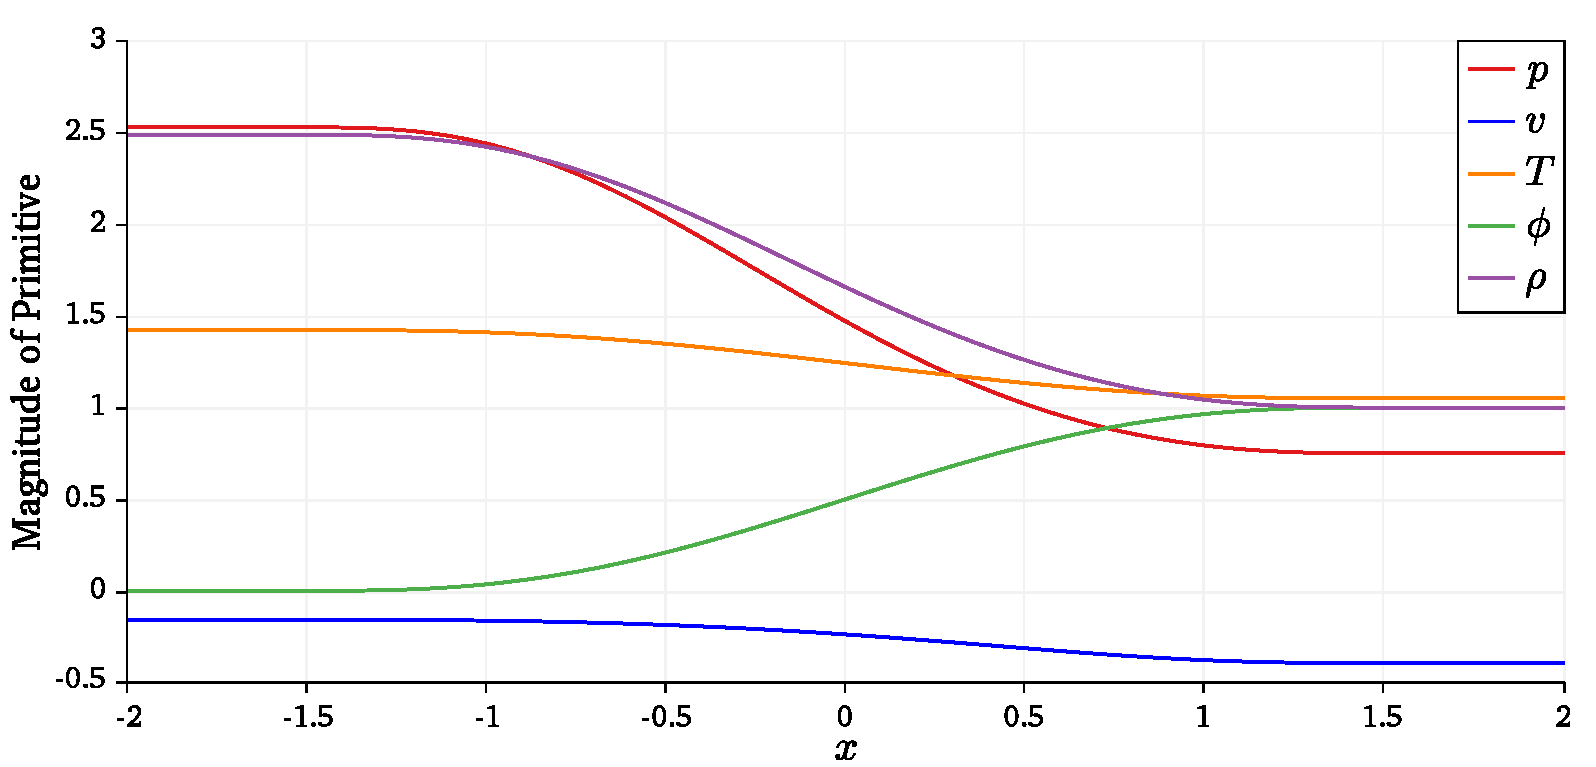
\includegraphics[width=13cm]{figures/OVS_initial_profile}
\caption {Magnitude profiles of the primitive values, density, and potential field at the initial time for the unperturbed equilibrium convergence test.}
\label{fig:OVS_initial_profile}
\end{figure}

Results of the simulations were characterized using the average absolute error magnitude, which is calculated as the normalized L1 norm of the error
\begin{equation}
Err_1=\frac{1}{N}\sum\limits_{i=1}^N \left|\rho_i-\rho_{i,\textrm{ref}}\right|,
\end{equation}
where $\rho_{\textrm{ref}}$ is a reference solution that is obtained either from exact calculation of the unperturbed equilibrium flow values, or from an overkill high-resolution simulation computed using $N=21870$ cells and the second-order well-balanced scheme for the test cases with the Gaussian perturbation. For the OVS, the number of cells is progressively tripled from $N=10$ to $N=7290$ and the intra-step order of accuracy is computed by determining the slope of the line connecting the error values of each adjacent pair of simulations using successively refined grids on a log-log plot of $Err_1$ vs.\ $\Delta x$.

Tripling was used such that when refining the grid, each cell would be perfectly split in three, and thus the position of the cell centre for the newly created middle cell would align exactly with the cell centre for the original coarse cell. Therefore, no interpolation is required to compare the cell centre values with the solutions obtained at any of the finer resolutions, and in particular the reference solution contains a value precisely at the location of each cell centre of every other grid resolution tested.

All convergence simulations were run to a final time of $t=1$, which was sufficient for the perturbations to have travelled significantly through the domain but still be most entirely contained within it.

\subsection{Equilibrium Flow}

The results of the first series of simulations at equilibrium, i.e.\ with $A=0$, are tabulated in Table~\ref{table:OVS_A0} and demonstrate very close agreement to the expected first- and second-order accuracy for the unbalanced schemes. For the well-balanced schemes, the average error is at the level of the machine precision for all grid resolutions, demonstrating the precise maintenence of the equilibrium flow irrespective of the number and size of the grid cells. This serves as a strong empirical verification of the precise matching between the source and flux term discretizations in the~\eqref{eq:balance} balance law for steady states, i.e.\ it truly is ``well-balanced''.

\begin{table*}\centering
\caption{L1 error of the density and intra-step order of accuracy for the first- and second-order unbalanced/well-balanced schemes with no perturbation, i.e.\ $A=0$.}
\ra{1.3}
\label{table:OVS_A0}
\begin{tabular}{@{}rcccccc@{}}\toprule
& \phantom{a} & \multicolumn{2}{c}{First} & \phantom{ab} & \multicolumn{2}{c}{Second}\\
\cmidrule{3-4} \cmidrule{6-7}
$N$ && $Err_1$ & Order && $Err_1$ & Order\\ \midrule
$10$ && 8.54e-02/4.04e-15 &&& 2.59e-02/4.04e-15 &\\
$30$ && 2.89e-02/5.20e-15 & 0.99/- && 3.16e-03/5.20e-15 & 1.91/-\\
$90$ && 9.77e-03/4.08e-15 & 0.99/- && 3.44e-04/4.09e-15 & 2.02/-\\
$270$ && 3.27e-03/3.63e-15 & 1.00/- && 3.77e-05/3.66e-15 & 2.01/-\\
$810$ && 1.09e-03/2.96e-15 & 1.00/- && 4.17e-06/5.05e-15 & 2.00/-\\
$2430$ && 3.64e-04/3.78e-14 & 1.00/- && 4.63e-07/5.20e-14 & 2.00/-\\
$7290$ && 1.21e-04/1.04e-14 & 1.00/- && 5.14e-08/1.37e-14 & 2.00/-\\
\bottomrule
\end{tabular}
\end{table*}

In Fig.~\ref{fig:OVS_A0} can be seen a visual representation of the same data from Table~\ref{table:OVS_A0}, making clear both the clean asymptotic convergence of the standard schemes as well as the many orders of magnitude greater accuracy achieved by the well-balanced method in simulating the stationary flow.

\begin {figure}
\centering
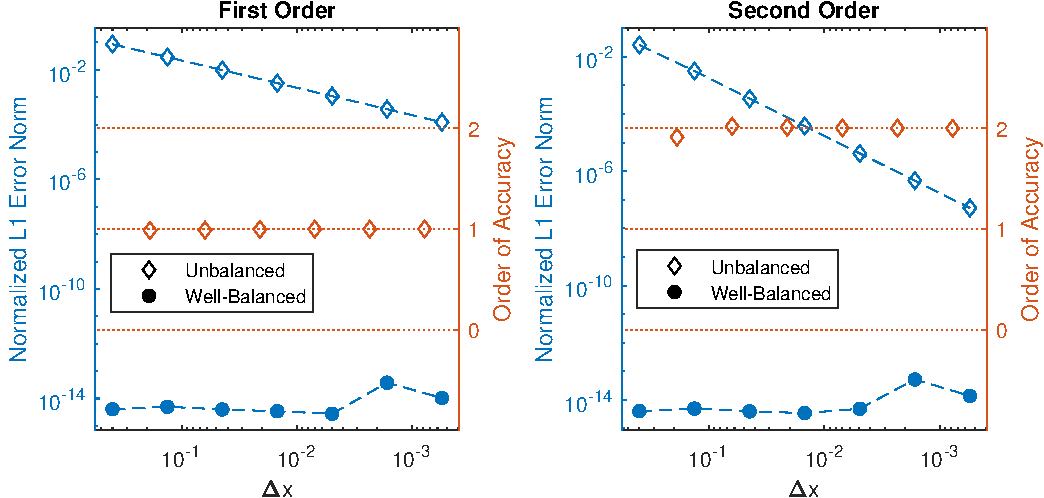
\includegraphics[width=13cm]{figures/OVSeps0}
\caption {L1 error of the density (in blue with dashed line) and intra-step order of accuracy (in red with no line) for the first- and second-order unbalanced and well-balanced schemes with no perturbation, i.e.\ $A=0$.}
\label{fig:OVS_A0}
\end{figure}

\subsection{Gaussian Perturbation}

Next is a series of tests using a `medium' amplitude Gaussian perturbation with $A=0.1$, with the initial and final density profiles of the reference solution shown in Fig.~\ref{fig:OVS_Amedium_profile}. This amplitude was chosen as it is large enough to be clearly resolved by all four combinations of first/second-order and un/well-balanced schemes, as seen in the table where all average errors are smaller than $A$. However, the amplitude was still small enough to ensure that the final solution remained smooth and does not yet present any steepening of flow features into discontinuities. Data from the convergence tests are presented in Table~\ref{table:OVS_Amedium} and visualized in Fig.~\ref{fig:OVS_Amedium}.

\begin {figure}
\centering
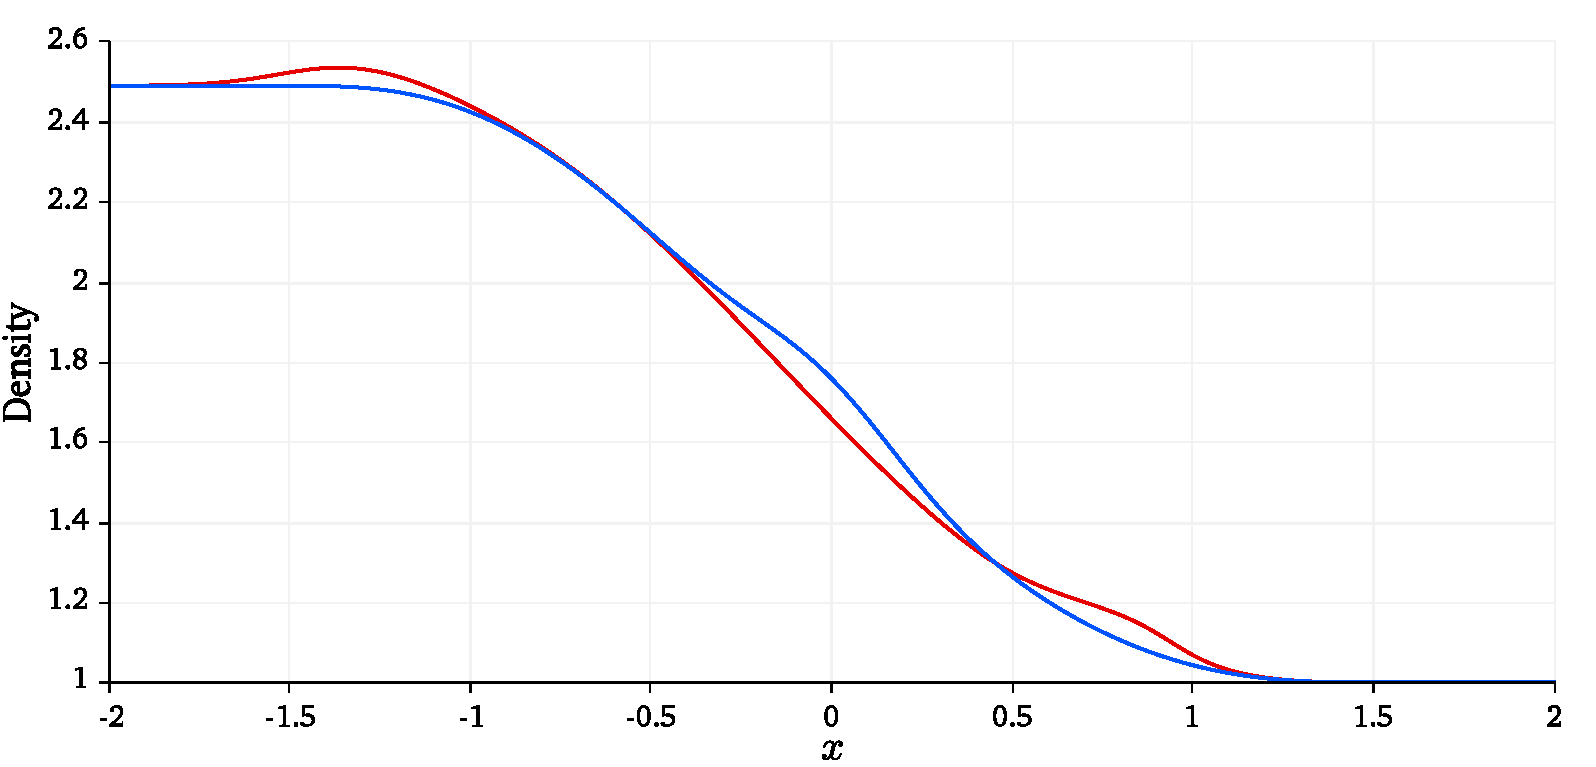
\includegraphics[width=13cm]{figures/OVSeps0_1profile}
\caption {Density profiles at the initial time (blue line) and final time (red line) of the reference simulation for the medium amplitiude $(A=0.1)$ convergence test, showing no discontinuities.}
\label{fig:OVS_Amedium_profile}
\end{figure}

It can be seen that the expected orders of accuracy are observed for the respective first- and second-order schemes where the graphs are in the asymptotic regime. In the second-order case it is noted that the results become abruptly non-linear for the smallest 1-2 grid spacings, due to the use of a reference solution which is itself only computed with the second-order well-balanced scheme using thrice as many cells as the final resolution presented on the plots. Thus the magnitude of errors still present in this reference becomes comparable to the errors in the final steps of the grid refinement, and so the linear convergence breaks down.

\begin{table*}\centering
\caption{L1 error of the density and intra-step order of accuracy for the first- and second-order unbalanced/well-balanced schemes with medium perturbation amplitude $A=0.1$.}
\ra{1.3}
\label{table:OVS_Amedium}
\begin{tabular}{@{}rcccccc@{}}\toprule
& \phantom{a} & \multicolumn{2}{c}{First} & \phantom{ab} & \multicolumn{2}{c}{Second}\\
\cmidrule{3-4} \cmidrule{6-7}
$N$ && $Err_1$ & Order && $Err_1$ & Order\\ \midrule
$10$ && 8.63e-02/1.23e-02 &&& 2.72e-02/7.51e-03 &\\
$30$ && 2.90e-02/9.68e-03 & 0.99/0.21 && 5.76e-03/3.78e-03 & 1.41/0.62\\
$90$ && 1.05e-02/5.63e-03 & 0.93/0.49 && 7.30e-04/5.29e-04 & 1.88/1.79\\
$270$ && 4.01e-03/2.61e-03 & 0.87/0.70 && 7.37e-05/5.34e-05 & 2.09/2.09\\
$810$ && 1.48e-03/1.01e-03 & 0.91/0.86 && 8.68e-06/5.89e-06 & 1.95/2.01\\
$2430$ && 5.14e-04/3.58e-04 & 0.96/0.95 && 2.97e-06/8.48e-07 & 0.98/1.76\\
$7290$ && 1.74e-04/1.22e-04 & 0.98/0.98 && 2.62e-06/5.80e-07 & 0.11/0.35\\
\bottomrule
\end{tabular}
\end{table*}

\begin {figure}
\centering
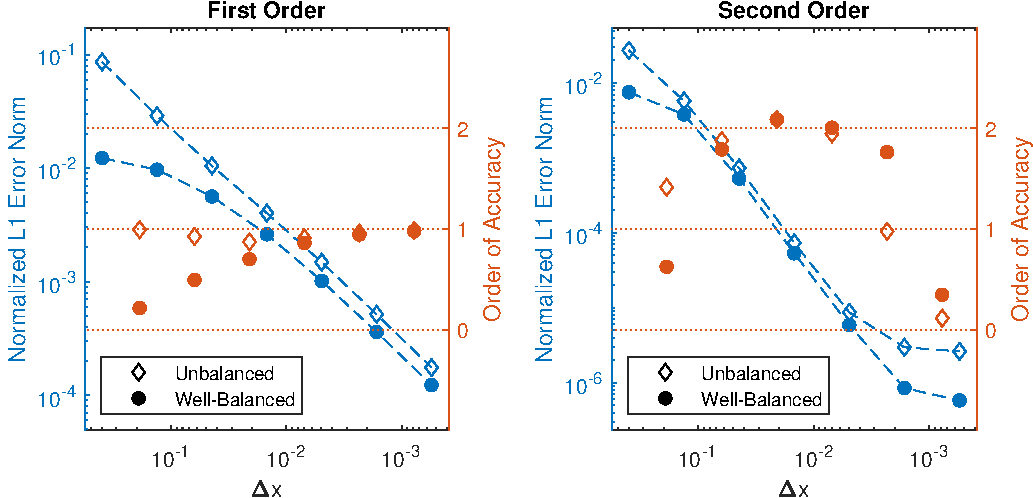
\includegraphics[width=13cm]{figures/OVSeps0_1}
\caption {L1 error of the density (in blue with dashed line) and intra-step order of accuracy (in red with no line) for the first- and second-order unbalanced and well-balanced schemes with medium perturbation amplitude $A=0.1$.}
\label{fig:OVS_Amedium}
\end{figure}

\subsection{Small Amplitude Perturbation}

In all cases for the medium amplitude, the well-balanced scheme is observed to have slightly lower errors than the unbalanced scheme, although the difference is relatively minor in this instance where the perturbation is much larger than the errors in the underlying equilibrium observed in the first convergence series with no perturbation. As such, we are interested in observing what happens for a perturbation amplitude that is quite small, comparable to or less than the average errors observed for the unbalanced scheme on the equilibrium flow. Therefore a third convergence series was carried out using a very small amplitude perturbation with $A=10^{-4}$, the results of which can be found in Table~\ref{table:OVS_Asmall} and Fig.~\ref{fig:OVS_Asmall}.

\begin{table*}\centering
\caption{L1 error of the density and intra-step order of accuracy for the first- and second-order unbalanced/well-balanced schemes with very small perturbation amplitude $A=10^{-4}$.}
\ra{1.3}
\label{table:OVS_Asmall}
\begin{tabular}{@{}rcccccc@{}}\toprule
& \phantom{a} & \multicolumn{2}{c}{First} & \phantom{ab} & \multicolumn{2}{c}{Second}\\
\cmidrule{3-4} \cmidrule{6-7}
$N$ && $Err_1$ & Order && $Err_1$ & Order\\ \midrule
$10$ && 8.54e-02/1.22e-05 &&& 2.59e-02/7.71e-06 &\\
$30$ && 2.89e-02/9.73e-06 & 0.99/0.21 && 3.17e-03/3.93e-06 & 1.91/0.61\\
$90$ && 9.77e-03/5.71e-06 & 0.99/0.49 && 3.44e-04/5.42e-07 & 2.02/1.80\\
$270$ && 3.27e-03/2.67e-06 & 1.00/0.69 && 3.77e-05/5.36e-08 & 2.01/2.11\\
$810$ && 1.09e-03/1.04e-06 & 1.00/0.86 && 4.17e-06/5.91e-09 & 2.00/2.01\\
$2430$ && 3.64e-04/3.67e-07 & 1.00/0.95 && 4.64e-07/8.39e-10 & 2.00/1.78\\
$7290$ && 1.21e-04/1.25e-07 & 1.00/0.98 && 5.28e-08/5.69e-10 & 1.98/0.35\\
\bottomrule
\end{tabular}
\end{table*}

\begin {figure}
\centering
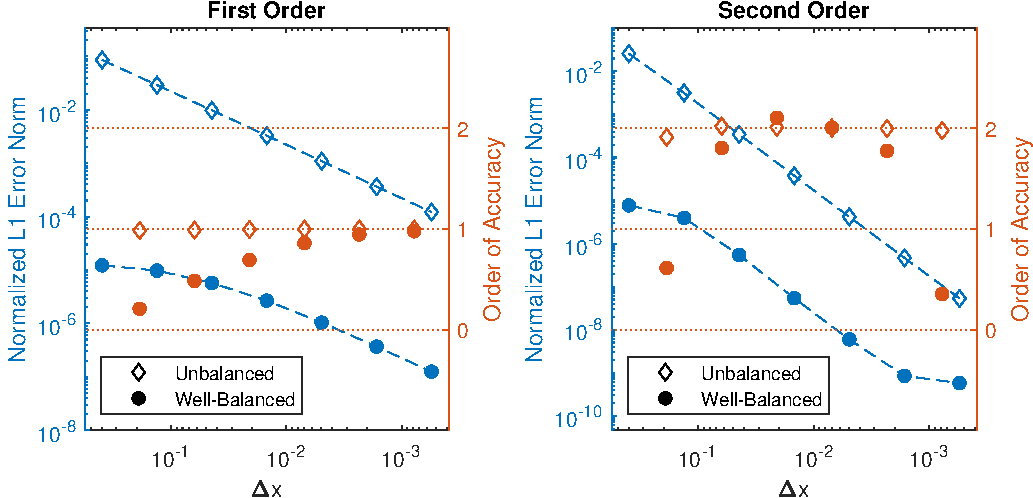
\includegraphics[width=13cm]{figures/OVSeps0_0001}
\caption {L1 error of the density (in blue with dashed line) and intra-step order of accuracy (in red with no line) for the first- and second-order unbalanced and well-balanced schemes with very small perturbation amplitude $A=10^{-4}$.}
\label{fig:OVS_Asmall}
\end{figure}

From the results, it is clear that the average error of the unbalanced scheme is much larger than the perturbation amplitude for all studied grid resolutions in the first-order case, and and even for the second-order scheme requires a fairly significant level of refinement before the error drops low enough for the perturbation to possibly be well resolved. The order of the convergence is of course still correct in both instances, but this is essentially just the same convergence towards the equilibrium as in the $A=0$ case, since the large magnitude of the errors compared to the perturbation amplitude mean that the deviation is not meaningfully percieved or simulated by the scheme over much of the parameter space.

By contrast, the well-balanced scheme exhibits average errors much smaller than the pertuabtion amplitude, with even the least resolved first-order simulation already having almost a full order of magnitude smaller error. Observed orders of convergence are the same as for the unbalanced scheme, but as exemplified visually in Fig.~\ref{fig:OVS_Asmall}, the absolute size of the errors is many orders of magnitude less for the well-balanced scheme. No level of grid refinement studied was able to get the first-order unbalanced scheme to the accuracy of its well-balanced counterpart, and it required approximately $3^3$ times more grid cells in the second-order tests to match the observed accuracy there. This demonstrates the potentially massive savings in computational cost provided by the well-balanced method for simulating small perturbations, especially in 2D or 3D simulations where the benefits would be compounded along each additional dimension.

\subsection{Discontinuous Flow}

Lastly, a large $A=2$ amplitude perturbation was used to investigate the performance of the schemes when steepened discontinuities become present in the solution. As seen in Fig.~\ref{fig:OVS_Alarge_profile}, the density profiles at the final time have developed clear discontinuities from the initially smooth profile. The results of the convergence tests for this amplitude are given in Table~\ref{table:OVS_Alarge} and reveal that the order of accuracy has now dropped to first-order for all schemes, because the gradient limiting means that the normally second-order schemes are reduced to first-order accuracy at the sharp transition points, and so this observed reduction in the convergence order agrees with the expected behaviour of such TVD limited reconstruction methods.

\begin {figure}
\centering
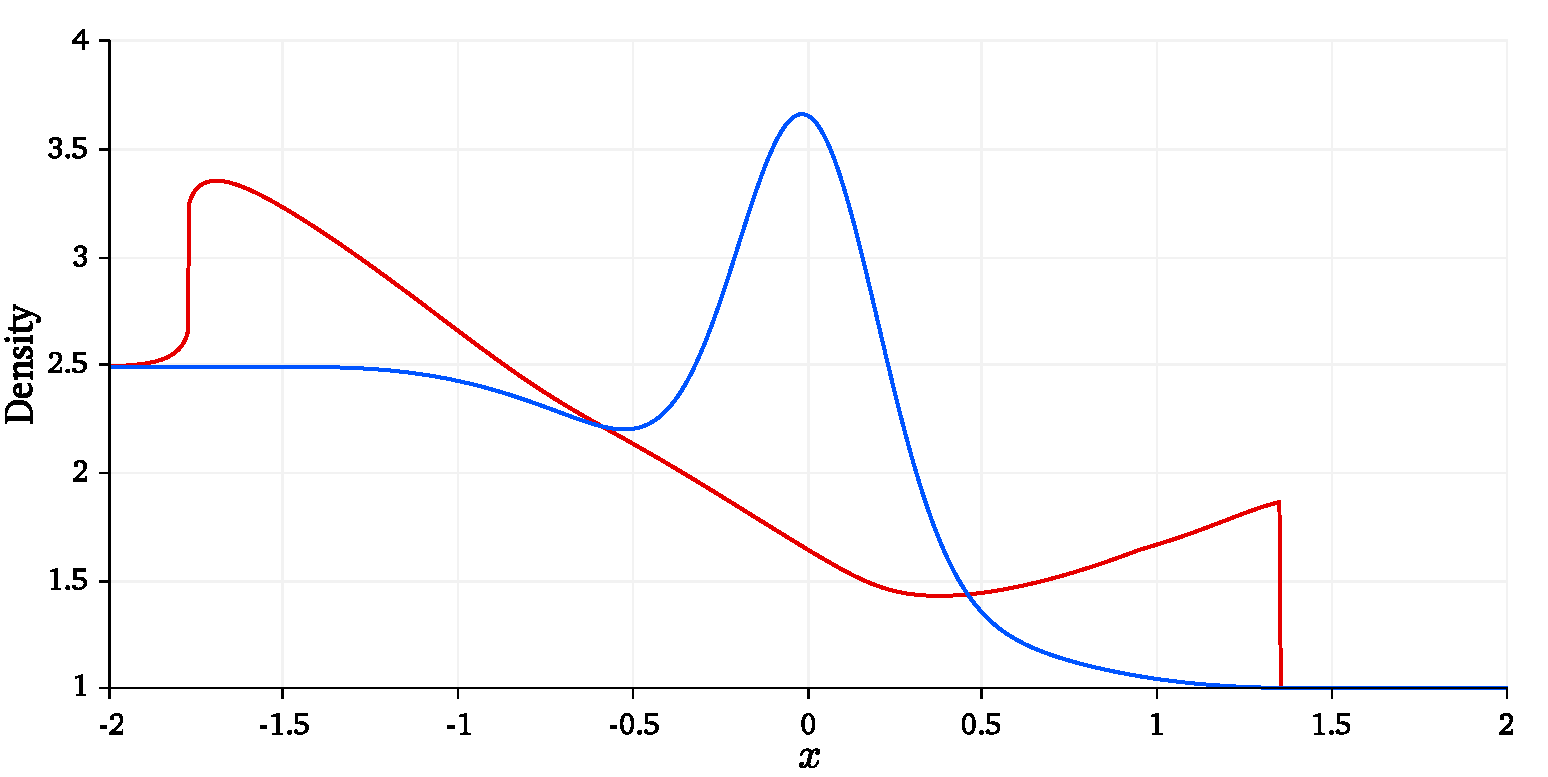
\includegraphics[width=13cm]{figures/OVSeps2profile}
\caption {Density profiles at the initial time (blue line) and final time (red line) of the reference simulation for the large amplitiude $(A=2)$ convergence test, showing clear discontinuities.}
\label{fig:OVS_Alarge_profile}
\end{figure}

Fig.~\ref{fig:OVS_Alarge} shows almost perfect overlap of the errors of the un/well-balanced schemes. Since the iterative Newton-Raphson solutions that are required by the balanced scheme will make it more computationally expensive than the standard method for a given grid resolution, and combined with the earlier medium and small amplitude results, this implies that the use of the well-balanced scheme is only justified for simulations involving deviations from the equilibrium flow that are smaller than or comparable to the error in the equilibrium state for the standard scheme. For such cases, the machine precision accuracy of the equilibrium for the balanced scheme means the perturbation can be simulated with a (potentially much) coarser grid, thus countering the higher computational cost per cell to result in overall savings of required effort for a given level of accuracy.

\begin{table*}\centering
\caption{L1 error of the density and intra-step order of accuracy for the first- and second-order unbalanced/well-balanced schemes with very large perturbation amplitude $A=2$.}
\ra{1.3}
\label{table:OVS_Alarge}
\begin{tabular}{@{}rcccccc@{}}\toprule
& \phantom{a} & \multicolumn{2}{c}{First} & \phantom{ab} & \multicolumn{2}{c}{Second}\\
\cmidrule{3-4} \cmidrule{6-7}
$N$ && $Err_1$ & Order && $Err_1$ & Order\\ \midrule
$10$ && 2.12e-01/1.96e-01 &&& 1.13e-01/1.13e-01 &\\
$30$ && 1.43e-01/1.44e-01 & 0.36/0.28 && 5.06e-02/5.10e-02 & 0.74/0.73\\
$90$ && 8.04e-02/7.93e-02 & 0.52/0.54 && 1.75e-02/1.75e-02 & 0.97/0.97\\
$270$ && 3.69e-02/3.66e-02 & 0.71/0.70 && 5.26e-03/5.26e-03 & 1.09/1.10\\
$810$ && 1.50e-02/1.48e-02 & 0.82/0.83 && 1.88e-03/1.88e-03 & 0.94/0.93\\
$2430$ && 5.88e-03/5.80e-03 & 0.85/0.85 && 5.86e-04/5.82e-04 & 1.06/1.07\\
$7290$ && 2.18e-03/2.15e-03 & 0.90/0.90 && 2.00e-04/1.83e-04 & 0.98/1.05\\
\bottomrule
\end{tabular}
\end{table*}

\begin {figure}
\centering
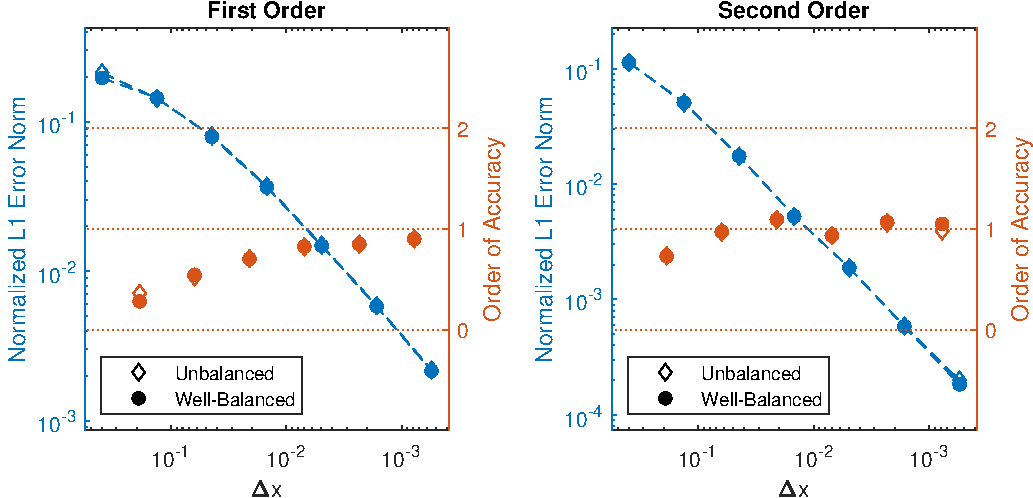
\includegraphics[width=13cm]{figures/OVSeps2}
\caption {L1 error of the density (in blue with dashed line) and intra-step order of accuracy (in red with no line) for the first- and second-order unbalanced and well-balanced schemes with large perturbation amplitude $A=2$.}
\label{fig:OVS_Alarge}
\end{figure}

For all amplitiudes, a good agreement is seen between the experimental results and the theoretically expected orders of accuracy, providing a solid verification of the correct implementation of the new well-balanced scheme.

\chapter{Application: SASI Toy Problem}
\label{chap:application}

As mentioned at the beginning of Chapter~\ref{chap:introduction}, the simple toy model of F09~\cite{Foglizzo2009} and SFF09~\cite{Sato2009} was chosen as a useful initial application of our well-balanced method to the SASI. The salient details from those papers are reproduced here.

The basic set-up of the problem consists of a 2D domain with periodic boundary conditions on both edges in the $x$-direction and three distinct flow regions in the $y$-direction. First is a supersonic inflow, which is transitioned by a shock front at $y=y_\textrm{sh}$ to subsonic speeds in the second region. This is then separated from a third region (also subsonic) by a potential step at $y=y_\nabla$ which further decelerates the flow and provides a simple model of matter slowing as it nears the surface of the accreting object. Following the notation of SFF09, we will denote quantities in the supersonic region before the shock with a subscript `1', in the interior region between the shock and potential step with `in', and in the outflow region past the step with `out'.

A schematic view of the problem domain with all three regions can be seen on the left side of Fig.~\ref{fig:Sato1}, with the right side showing how the overall scenario is then split into two sub-problems for initial simulation. This separation greatly simplifies the introduction of specific advective and acoustic perturbations to appropriate locations in the interior of the domain, making it much easier to see the interactions of these disturbances at the boundaries (the shock and potential step) between the various flow regions. Overall, this provides a much simplified analogue for simulations to study the mechanisms at play during the inflow, decceleration, and accretion of matter in a collapsing star before supernova.

\begin{figure}
\centering
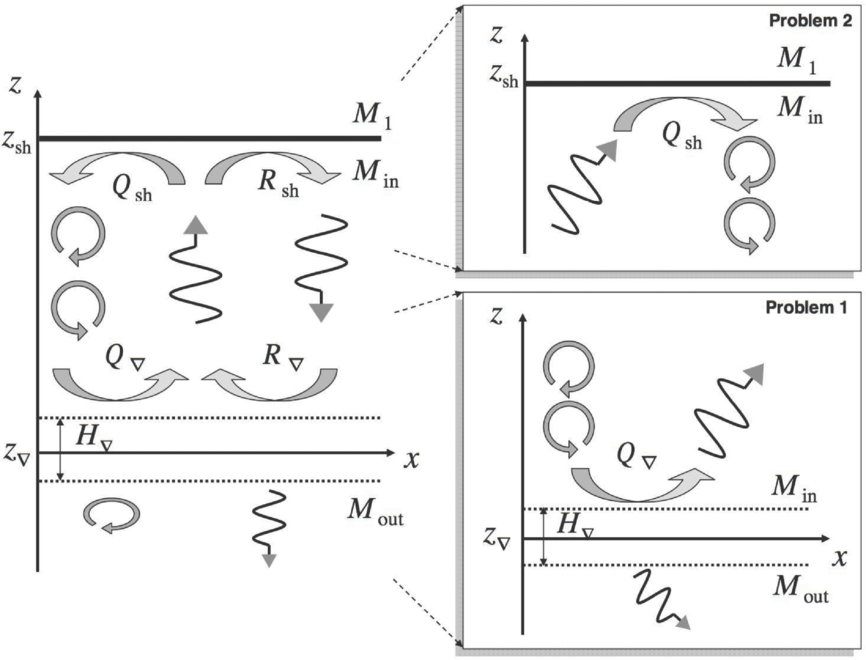
\includegraphics[width=13cm]{figures/Sato1}
\caption {This image is taken directly from SFF09~\cite{Sato2009}. On the left is a schematic diagram of the full toy problem for the SASI,  which is then broken into two sub-problems on the right. Circular arrows represent advective vorticity waves while wavy arrows denote acoustic pressure waves. The coupling efficiencies denote the strength of coupling between acoustic and advective waves ($Q_\textrm{sh}$, $Q_\nabla$) and the reflection of purely acoustic waves ($R_\textrm{sh}$, $R_\nabla$).}
\label{fig:Sato1}
\end{figure}

General parameters of the model problem will be presented next, followed by specific information for the potential step and stationary shock, computed separately as sub-problems 1 and 2, respectively. 


\section{Problem Set-up}
\label{sec:TP_set_up}

The general flow problem to be studied is essentially a 1D flow when at equilibrium, with the periodicity in the $x$-direction mimicking an infinitely wide flow and all variation occuring in the $y$-direction. Simulating this problem in 2D then, is done purely for studying the perturbations to this equilibrium flow, thus allowing more interesting perturbations and potential higher-dimenensional features to also be realized.

An ideal gas with an adiabatic constant $\gamma=4/3$ was simulated, the extent of the domain in the $x$-direction is denoted as $L_x$, and the entropy of the fluid is defined as
\begin{equation}
S\equiv\frac{\log\left(p/\rho^\gamma\right)}{\gamma-1}.
\end{equation}
Beginning with a Mach number of $\mathcal{M}_1=5$ at the inflow, one can then compute the relations of flow values across the shock as defined by the Rankine-Hugoniot conditions
\begin{equation}
\mathcal{M}_\textrm{in}=\sqrt{\frac{2+(\gamma-1)\mathcal{M}_1^2}{2\gamma\mathcal{M}_1^2-\gamma+1}},
\end{equation}
\begin{equation}
\frac{v_1}{v_\textrm{in}}=\frac{(\gamma+1)\mathcal{M}_1^2}{2+(\gamma-1)\mathcal{M}_1^2},
\end{equation}
\begin{equation}
\frac{\rho_1}{\rho_\textrm{in}}=\frac{v_\textrm{in}}{v_1},
\end{equation}
where $v_\textrm{in}=-\mathcal{M}_\textrm{in}c_\textrm{in}$ and the interior Mach number is found to be $\mathcal{M}_\textrm{in}=\sqrt{31/199}\approx0.39$.

A hyperbolic tangent function is used to provide a smooth step-like external potential field centred at $y_\nabla=0$ extant over an approximate width $H_\nabla$, with the exact function given by
\begin{equation}
\phi(y)=\frac{\Delta\phi}{2}\left[\tanh\left(\frac{y-y_{\nabla}}{H_{\nabla}/2}\right)+1\right],
\end{equation}
where the step size $\Delta\phi$ is set based on the ratio of the sound speeds $c_{\textrm{in}}/c_{\textrm{out}}$ in the constant regions surrounding the step, and can be computed as
\begin{equation}
\Delta\Phi=\left(\frac{\mathcal{M}_\textrm{out}^2}{2}+\frac{1}{\gamma-1}\right)c_\textrm{out}^2-\left(\frac{\mathcal{M}_\textrm{in}^2}{2}+\frac{1}{\gamma-1}\right)c_\textrm{in}^2.
\end{equation}
For all simulations, the ratio $c_\textrm{in}^2/c_\textrm{out}^2=0.75$ was used, and the step width was chosen such that $H_\nabla/H=0.1$ where $H\equiv y_\textrm{sh}-y_\nabla$ is defined to be the distance between the shock and the middle of the potential step.

A reference timescale for the advective-acoustic cycle is used to normalize the simulation times, and is calculated as
\begin{equation}
\tau_\textrm{aac}\equiv\frac{1}{1-\mathcal{M}_\textrm{in}}\frac{H}{|v_\textrm{in}|}.
\end{equation}
Units for all quantities are chosen to ensure that $c_\textrm{in}=\rho_\textrm{in}=H=1$. Using the relation $p=\rho c^2/\gamma$ we can compute the other primitive values in the interior region as $p_\textrm{in}=0.75$ and $T_\textrm{in}=1.05$ and the reference timescale as $\tau_\textrm{aac}\approx4.2$. A wavenumber $k_x=2\pi/L_x$ is used to define linear perturbations of the flow, where $L_x=4$, along with a temporal frequency defined as $\omega_0=4\pi/\tau_\textrm{aac}$.

For both sub-problems a $4\times4$ square domain is used, divided into a uniform number $N_x=N_y=400$ of square grid cells in both dimensions. This gives a uniform grid spacing of $\Delta x=\Delta y=10^{-2}$.

\subsection{Sub-Problem 1: Potential Step}
\label{subsec:sub_problem_1}

For the first sub-problem, the potential step positioned at $y_\nabla=0$ is the only flow feature simulated on a square domain defined on $y\in[-1,3]$, $x\in[0,4]$. Inflow occurs at the upper $y=3$ boundary, defined using Dirichlet conditions, and zero-gradient conditions are imposed at the $y=-1$ outflow boundary. Initial conditions are determined by computing the equilibrium flow for the given inlet primitive values over the potential field. By defining also a vertical wavenumber $k_y=\omega_0/v_\textrm{in}$ the perturbations injected at the inlet are given by the equations
\begin{equation}
\delta S\equiv\epsilon_S\cos\left(-\omega_0t+k_xx+k_yy\right),
\end{equation}
\begin{equation}
\frac{\delta \rho}{\rho_\textrm{in}}\equiv\exp\left(-\frac{\gamma-1}{\gamma}\delta S\right)-1,
\end{equation}
where $\epsilon_S=10^{-3}$ is the amplitude of the generated entropy waves.

These incoming waves are desired to be at pressure equilibrium ($\delta p=0$), and so from the equation of state one can then determine the consistent temperature perturbation
\begin{equation}
\frac{\delta T}{T_\textrm{in}}=\left(1+\frac{\delta\rho}{\rho_\textrm{in}}\right)^{-1}-1=\exp\left(\frac{\gamma-1}{\gamma}\delta S\right)-1.
\end{equation}
Deviations to the 2D velocity components are given as
\begin{equation}
\delta v_x\equiv\frac{k_x\omega_0c_\textrm{in}^2}{\omega_0^2+k_x^2v_\textrm{in}^2}\frac{\delta S}{\gamma} \quad \textrm{and} \quad \delta v_y\equiv-\frac{k_x^2v_\textrm{in}c_\textrm{in}^2}{\omega_0^2+k_x^2v_\textrm{in}^2}\frac{\delta S}{\gamma},
\end{equation}
which result in the generation of the following vorticity waves 
\begin{equation}
\delta w_y=-\frac{k_xc_\textrm{in}^2}{v_\textrm{in}}\frac{\epsilon_S}{\gamma}\sin\left(-\omega_0t+k_xx+k_yy\right).
\end{equation}
These waves, which are injected only at the inlet, are allowed to travel through the interior region towards the potential step, and then any resultant coupling of the vorticity waves into reflected pressure waves is observed.

\subsection{Sub-Problem 2: Standing Shock}
\label{subsec:sub_problem_2}

For the second sub-problem, only the shock front positioned at $y_\textrm{sh}=1$ is simulated, with the square domain now defined on $y\in[-2,2]$, $x\in[0,4]$. Inflow is now supersonic and again set with Dirichlet boundaries at $y=2$, although the outflow conditions at $y=-2$ are different from sub-problem 1. Homogoneous Neumann conditions are still used initially while no perturbations are present in the system, to allow the shock to ``settle in'' and any waves generated by this settling process to propagate cleanly out of the system. Once a steady state is reached, however, the outflow conditions are changed to be also Dirichlet in order to inject the desired perturbations into the domain from the outflow boundary. The time at which this ``switching on'' of the injected perturbations occurs is labeled as the starting time $\tau=0$ for the simulations. Initial conditions are in this case determined purely by the Rankine-Hugoniot conditions given earlier to define the shock, since the potential field is now constant throughout the entire domain.

Vorticity-free pressure perturbations are generated for this sub-problem, and by defining a new vertical wavenumber
\begin{equation}
k_y^\pm=\frac{\omega_0}{c_\textrm{in}}\frac{\mathcal{M}_\textrm{in}\mp\mu}{1-\mathcal{M}_\textrm{in}^2},
\end{equation}
and density perturbation amplitude $\epsilon_\rho=10^{-3}$, one has the equations for the perturbations injected at the outlet as
\begin{align}
\frac{\delta\rho}{\rho_\textrm{in}}&\equiv\left(\frac{1+\mu\mathcal{M}_\textrm{in}}{1-\mathcal{M}_\textrm{in}^2}\right)\epsilon_\rho\cos\left(-\omega_0t+k_xx+k_y^-y\right), \\
\frac{\delta p}{p_\textrm{in}}&\equiv\left(1+\frac{\delta\rho}{\rho_\textrm{in}}\right)^\gamma-1,
\end{align}
where one can again use the equation of state to determine the consistent temperature deviation
\begin{equation}
\frac{\delta T}{T_\textrm{in}}=\left(1+\frac{\delta\rho}{\rho_\textrm{in}}\right)^{\gamma-1}-1.
\end{equation}
Velocity perturbations for these purely acoustic pressure waves are given by
\begin{align}
\delta v_x&\equiv\left(\frac{k_xc_\textrm{in}^2}{\omega_0}\right)\epsilon_\rho\cos\left(-\omega_0t+k_xx+k_y^-y\right), \\
\delta v_y&\equiv\left(\frac{\mu+\mathcal{M}_\textrm{in}}{1-\mathcal{M}_\textrm{in}^2}\right)c_\textrm{in}\epsilon_\rho\cos\left(-\omega_0t+k_xx+k_y^-y\right),
\end{align}
where the parameter $\mu$ is simply used for convenience and expands as
\begin{equation}
\mu\equiv\sqrt{1-\frac{k_x^2c_\textrm{in}^2}{\omega_0^2}\left(1-\mathcal{M}_\textrm{in}^2\right)}.
\end{equation}
These waves then propagate towards the shock front, and any resultant generation of reflected vorticity waves is measured.


\section{Numerical Results}
\label{sec:TP_results}

Results of simulations for the two sub-problems are presented next, comparing the results to those obtained in F09 and SFF09.

\subsection{Sub-Problem 1}
\label{subsec:results_TP1}

In Fig.~\ref{fig:TP1} can be seen the numerical results obtained for the potential step problem using the well-balanced scheme, with data presented in a manner similar to Fig.~2 in SFF09 to allow easy comparison. At three successive times, the first before and the second and third after the injected entropy/vorticity waves have reached the potential step, are shown the specific vorticity on the left and the normalized pressure perturbation on the right. Excellent qualitative agreement is seen to the corresponding figure in SFF09. Before the incident wave reaches the step, the right hand column is largely free of any perturbations, with reflected and (less strong) transmitted pressure deviations observed only as the incident wave passes through the deceleration zone centred at $y_\nabla=0$, illustrating clear generation of acoustic waves as the incoming vorticity wave is decelerated at the potential step. It is also clear to see that in comparison to the figure in SFF09, there is essentially no spurious deviation from the equilibrium flow observed over the potential step itself in our simulation with the new well-balanced scheme, at any of the timepoints.

\begin{figure}
\centering
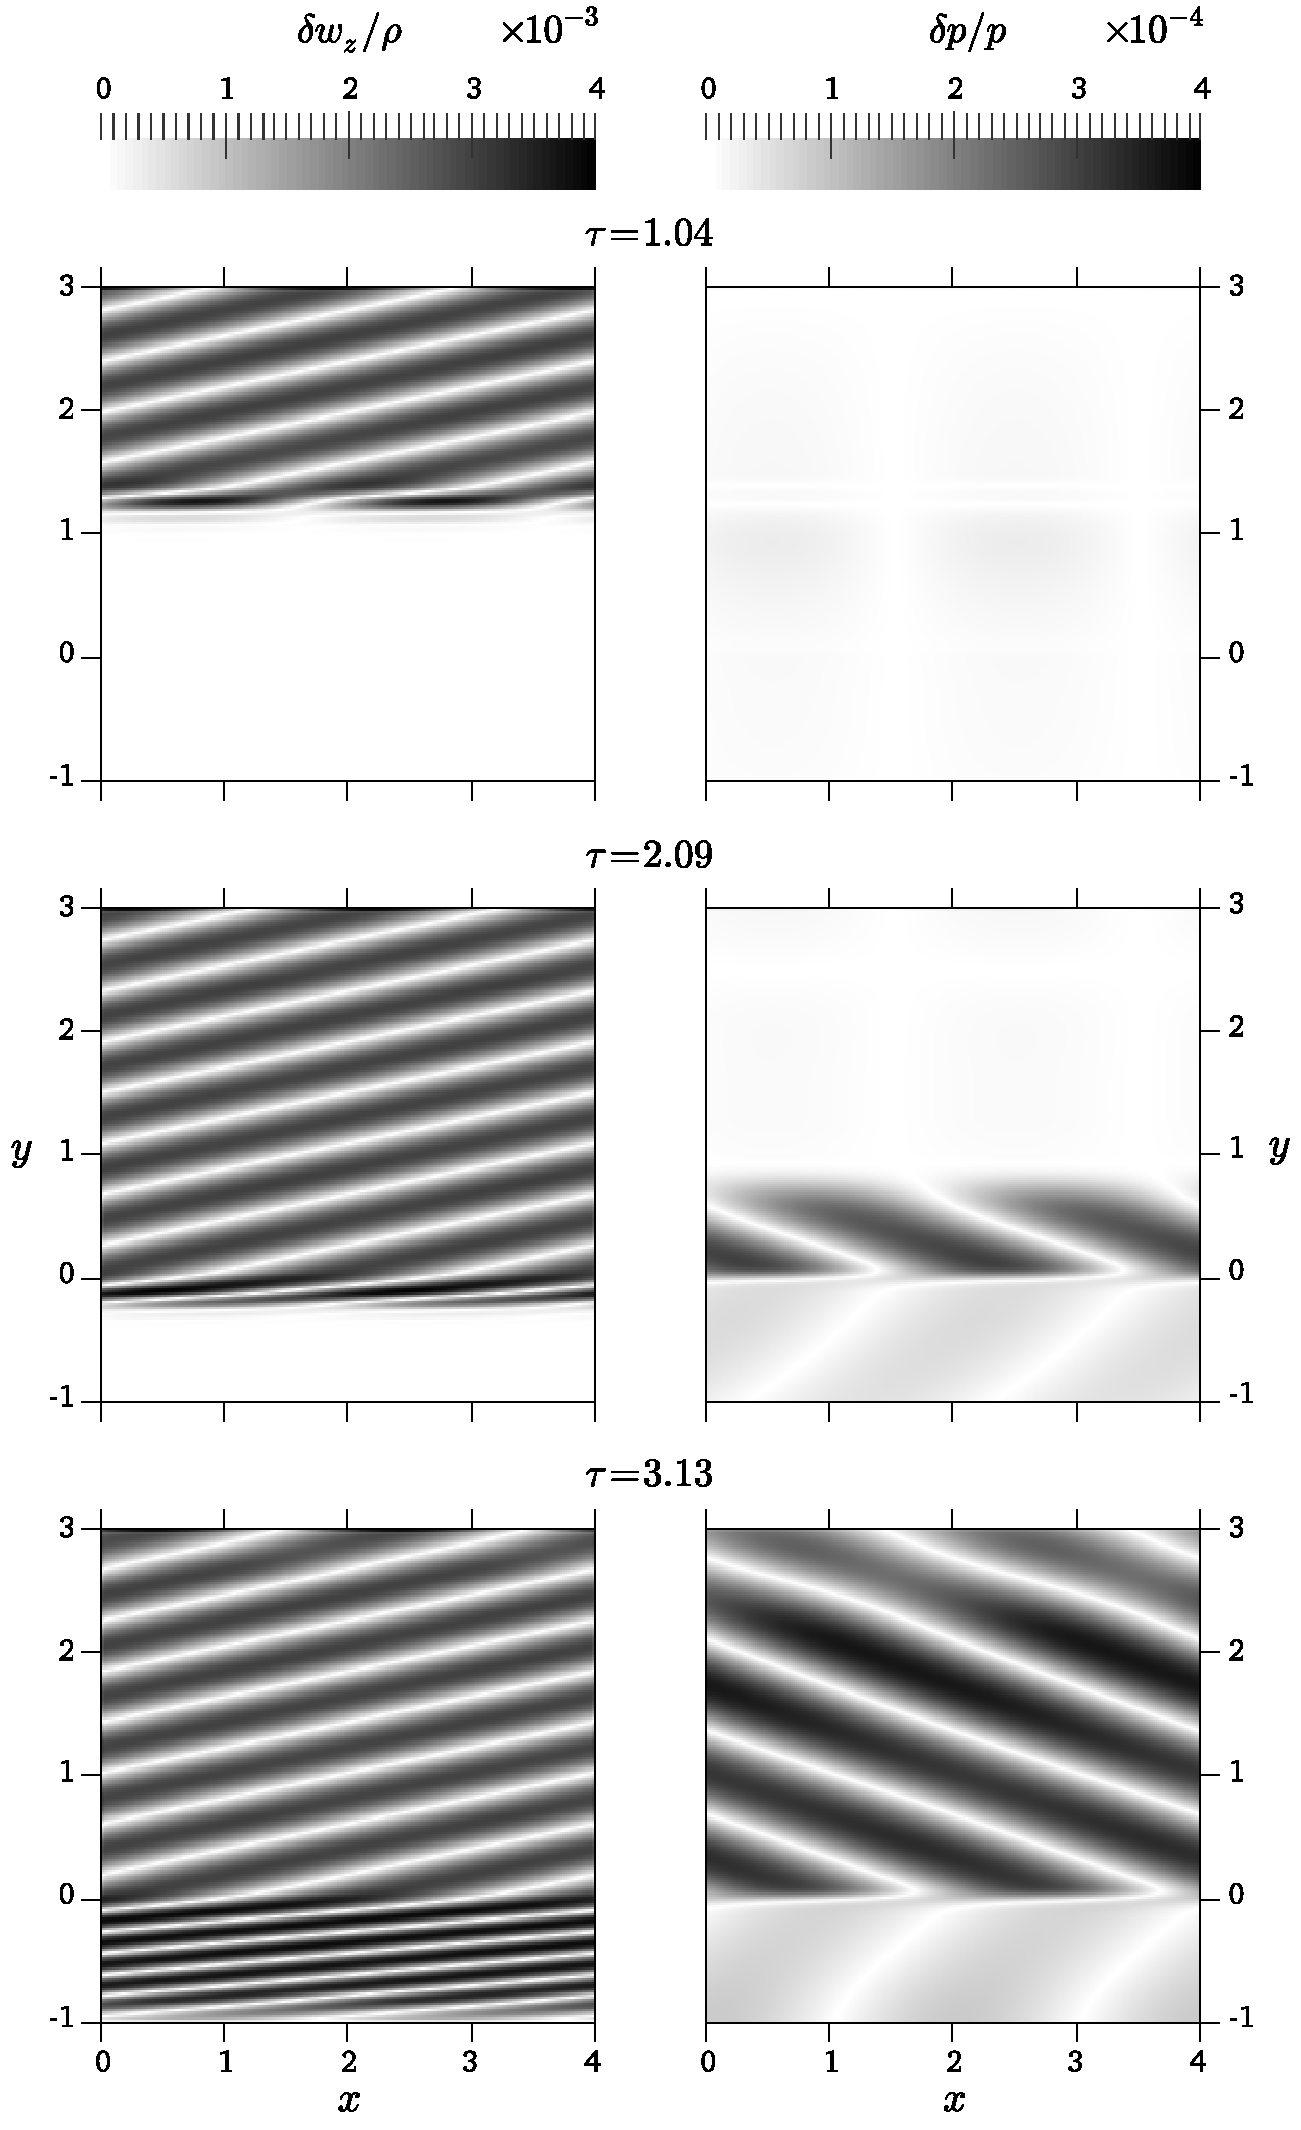
\includegraphics[width=12cm]{figures/TP1}
\caption {Results of sub-problem 1 which can be compared to Fig.~2 in SFF09~\cite{Sato2009}. Generation of an acoustic wave by the deceleration of a vorticity wave through a potential step centred at $y_\nabla=0$ is shown at three successive times $\tau$, normalized by $\tau_\textrm{aac}$.}
\label{fig:TP1}
\end{figure}

In order to obtain a more quantitative comparison, the amplitude of the acoustic feedback was measured, using a Fourier transform of the induced pressure perturbation, over one full wave period $T\equiv2\pi/\omega_0$, with the transform defined by
\begin{equation}
\hat{\delta p}_0=\frac{2}{T}\int\limits_{0}^{T}\delta pe^{i\omega_0t}\textrm{d}t.
\end{equation}
By assuming that the generated acoustic wave is advected away from the potential step relatively unchanged, in essence invoking Taylor's frozen turbulence hypothesis, the data for the perturbation was taken from the final timepoint ($\tau=3.13$) by measuring over a full spatial wavelength. These values are then cast back to the time domain by pairing the datapoints with the correct Fourier frequencies for the integration, as if they had in fact been taken at a single spatial point over the above time interval. With this, the efficiency of the acoustic feedback from the incoming entropy wave is calculated to be $$\left(\hat{\delta p}_0/p_\textrm{in}\right)/\delta S=0.338.$$
In order to have a good value for comparison, the expected value was read off the analytic solution line of Fig.~3 in SFF09 for the simulated frequency of $\omega_0\tau_\textrm{aac}/2\pi=2$ and determined to be approximately $\left(\hat{\delta p}_0/p_\textrm{in}\right)/\delta S=0.32$. This therefore shows excellent agreement between our simulated results and the expected value from the linear analysis undertaken in F09.

\subsection{Sub-Problem 2}
\label{subsec:results_TP2}

For the standing shock sub-problem, the results of the well-balanced simulation are shown in Fig.~\ref{fig:TP2}, here presented to allow easy comparison with Fig.~4 in SFF09. Data is again shown for three successive timepoints, in this instance before and after a pressure wave, injected at the outflow, reaches the shock front. Once there, it produces coupled vorticity/entropy perturbations back into the interior region, with excellent qualitative agreement for the advective-acoustic wave cycling observed with the respective figure in SFF09.

While there are a few very small spurious deviations visible in the specific vorticity (shown in the left hand column of the figure) in the immediate vicinity of the the shock throughout the simulation, the domain is predominantly vorticity-free before the incident wave reaches the shock. Only after the pressure wave, visible in the normalized pressure deviation shown in the right hand column of the figure, impacts the shock is clear generation of advective waves observed. This provides evidence for the necessary second half of the advective-acoustic cycle, complementing the generation of vorticity waves from incident pressure waves at the potential step observed in sub-problem 1.

\begin{figure}
\centering
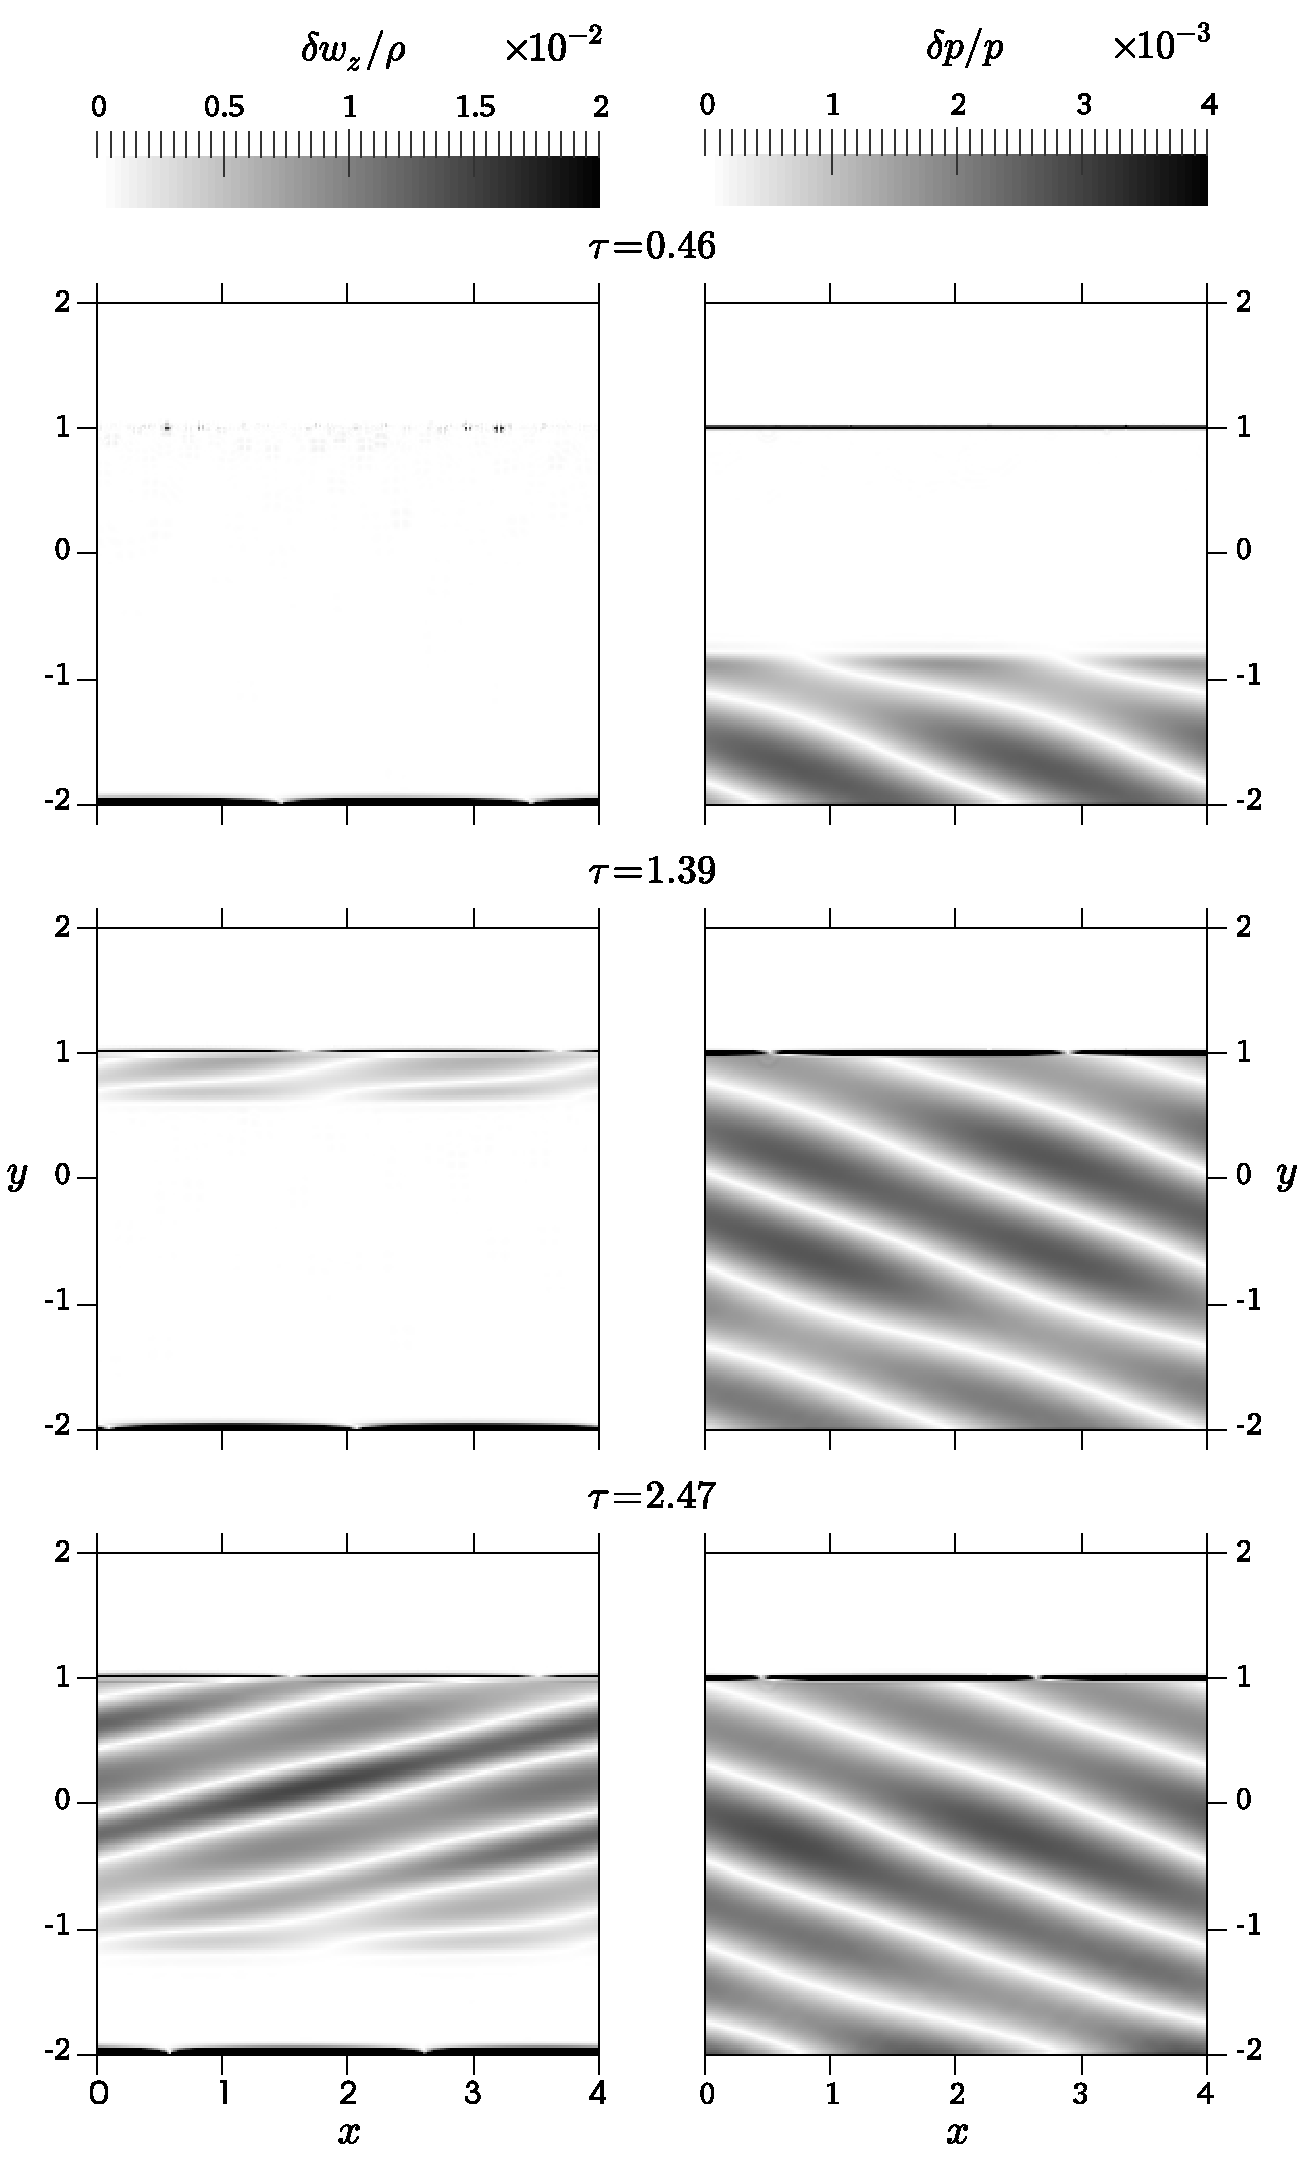
\includegraphics[width=12cm]{figures/TP2}
\caption {Results of sub-problem 2 which can be compared to Fig.~4 in SFF09~\cite{Sato2009}. Generation of a vorticity wave by the reflection of an acoustic wave from a shock located at $y_{\textrm{sh}}=1$ is shown at three successive times $\tau$, normalized by $\tau_\textrm{aac}$.}
\label{fig:TP2}
\end{figure}

To once again have a more quantitative check of the results in addition to the qualitative agreement with SFF09 observed above, the amplitude of the resulting entropy wave was measured for comparison to the expected value from theory. This theoretical value can be computed directly according to the formula from SFF09
\begin{equation}
\delta S_\textrm{th}=\frac{\delta p}{p_\textrm{in}}\frac{2}{\mathcal{M}_\textrm{in}}\frac{1-\mathcal{M}_\textrm{in}^2}{1+\gamma\mathcal{M}_\textrm{in}^2}\left(1-\frac{\mathcal{M}_\textrm{in}^2}{\mathcal{M}_1^2}\right)\frac{\mu}{\mu^2+2\mu\mathcal{M}_\textrm{in}+\mathcal{M}_1^{-2}},
\end{equation}
and for the given simulation is found to be $\delta S_\textrm{th}=3.28\textrm{e-}3$.

Analyzing the results of the numerical simulation at the final timetep from the figure, $\tau=2.47$, the amplitude of the generated entropy wave is measured to be $$\delta S_\textrm{sim}=2.94\textrm{e-}3.$$ This once again demonstrates relatively good agreement between the results obtained using the newly implemented well-balanced method and the theoretically expected value determined from the analytic treatment of F09 and SFF09.

With both parts of the advective-acoustic cycle thus independently observed, it remains to then put the two sub-problems together for a simulation of both effects concurrently.

\subsection{Full Toy Problem}
\label{subsec:results_TP}

The complete toy problem was simulated, with both the standing shock and the potential step now present in the domain simultaneously. Perturbations to the density and pressure equilibria were introduced in the supersonic inflow region to mimic spatial inhomogeneities which could be present in the distribution of accreting matter prior to a core-collapse supernova.

Keeping the same horizontal wavenumber $k_x=2\pi/L_x$ but defining a new vertical wavenumber as $k_y=\omega_0/v_1$ and density perturbation amplitude as $\epsilon_\rho=10^{-4}$ we have the following equations for the density and pressure perturbations at the supersonic inflow
\begin{equation}
\delta\rho=\epsilon_\rho\cos\left(-\omega_0t+k_xx+k_yy\right),
\end{equation}
\begin{equation}
p=p_1+\delta p=(\rho_1+\delta\rho)RT_1,
\end{equation}
where $R$ is the specific gas constant and the velocity and temperature are kept at constant equilibrium ($\delta v=\delta T=0$).

Initial conditions were set by splicing together the ``settled in'' initial conditions used for the shock in sub-problem 2 with the analytically computed equlibrium used for the sub-problem 1 initial conditions, with the join occuring just below the shock at $y=0.92$. For all quantities Dirichlet boundary conditions were imposed at the inlet with homogenous Neumann conditions used at the outflow.

The simulation was allowed to progress to a final time of $\tau=3$ (normalized by $\tau_{aac}$) where the time origin $\tau=0$ was set to be the time just before the incoming perturbations impacted on the shock front. Measurements of the maximal perturbation amplitudes were taken in the interior region between the shock and the potential step, $y\in[0.1,0.9]$, and these values are tabulated in Table~\ref{table:TP} for several key timepoints. Visual results for three of these timepoints are also shown in Fig.~\ref{fig:TP} for comparison.

\begin{table*}\centering
\caption{Maximum amplitudes of the specific advective and acoustic perturbations in the interior region between the shock and potential step at successive times $\tau$, normalized by $\tau_\textrm{aac}$.}
\ra{1.3}
\label{table:TP}
\begin{tabular}{@{}lcccc@{}}\toprule
& \phantom{abc} & \multicolumn{3}{c}{Perturbation Amplitude} \\
\cmidrule{3-5}
\phantom{al}$\tau$ && $\delta w_z/\rho$ & \phantom{abc} & $\delta p/p$ \\
\midrule
$0.125$ && 2.99e-03 && 2.83e-04 \\
$0.500$ && 3.23e-03 && 4.01e-04 \\
$1.00$ && 3.65e-03 && 6.65e-04 \\
$2.00$ && 5.21e-03 && 8.12e-04 \\
$3.00$ && 5.95e-03 && 8.89e-04 \\
\bottomrule
\end{tabular}
\end{table*}

\begin{figure}
\centering
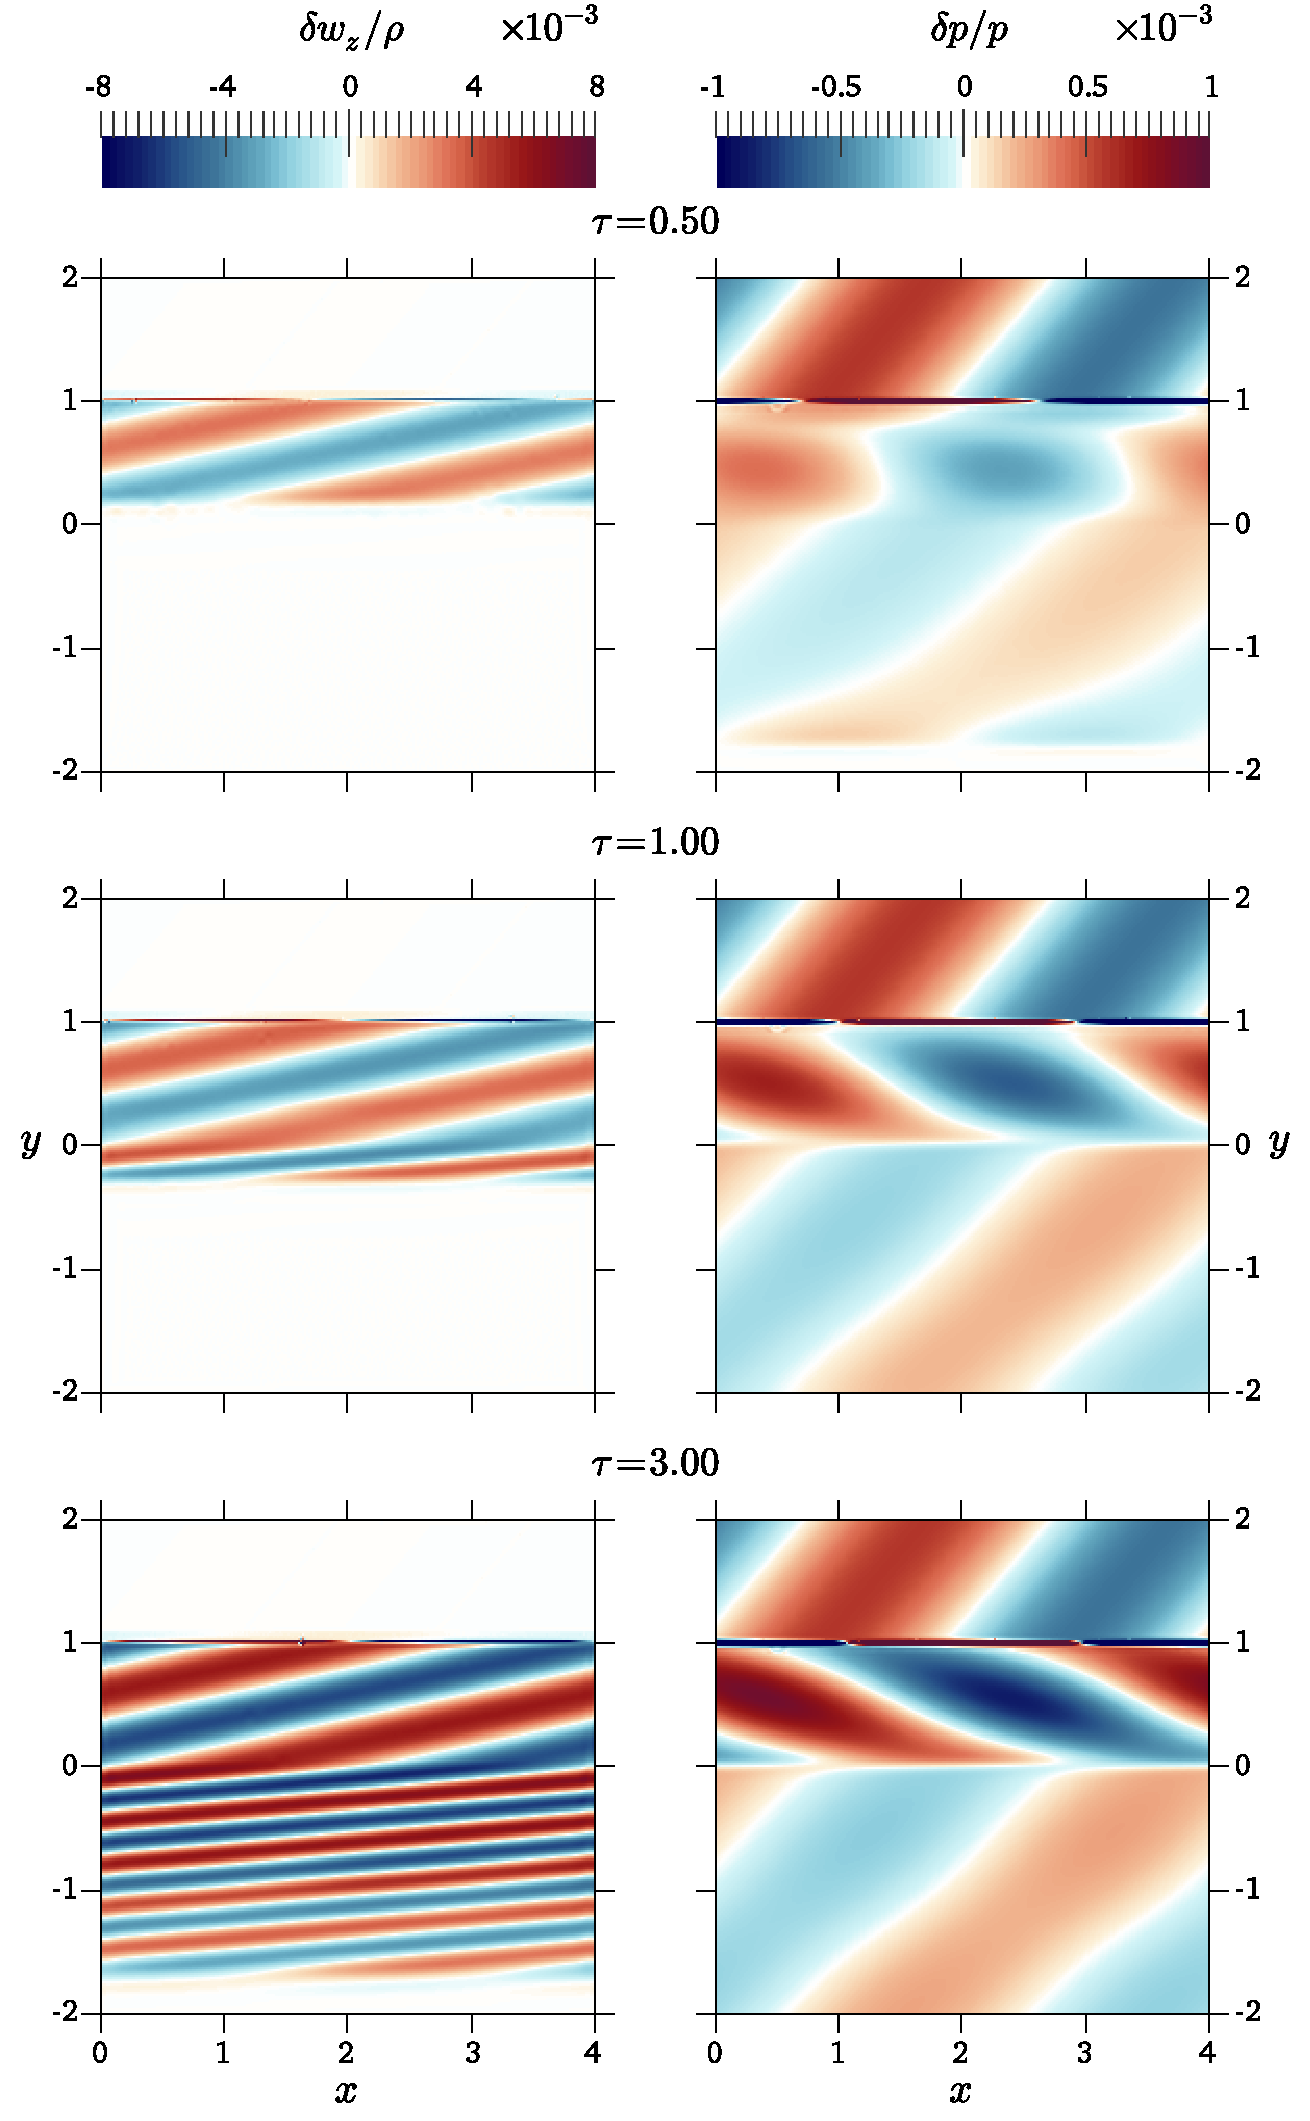
\includegraphics[width=12cm]{figures/TP}
\caption {Results of the full toy problem simulation, showing the advective-acoustic cycle. Coupling of vorticity and pressure waves at both a shock located at $y_{\textrm{sh}}=1$ and a potential step located at $y_\nabla=0$ is shown at three successive times $\tau$, normalized by $\tau_\textrm{aac}$.}
\label{fig:TP}
\end{figure}

At the first time given in the table, $\tau=0.125$ (not shown in figure), the incident perturbations have reached the shock and resultant perturbations in both the pressure and vorticity are observed being generated and travelling into the interior region. Neither of these wave types have yet reached the potential step at this point, and so the amplitudes given in the table represent purely the strength of the coupling from the injected perturbations in the supersonic inflow.

Moving to the second time in the table, $\tau=0.5$ (top row of figure), the faster moving acoustic wave has now reached the potential step, with part of the energy being transmitted through to the outflow and part reflected back into the interior, with the amplitude for the specific pressure perturbation observed to increase noticeably. By contrast, the slower moving advective wave has not yet reached the potential step, and no coupling of acoustic to advective waves is observed at the potential step, and so the measured amplitude of the specific vorticity perturbations has not increased by much from the initial value.

At $\tau=1$ (middle row of figure), the advective wave has now also reached the potential step, and coupled reflection of acoustic waves back into the interior region is observed, and is evidenced by another significant increase in the measured amplitude of the specific pressure deviation. No reflection of these advective perturbations is observed, of course, but some transmission of vorticity into the outflow can be clearly seen. A small increase in the specific vorticity perturbation amplitude is measured, due to the coupling at the shock of the acoustic reflections from the potential step noted previously at $\tau=0.5$, but the much larger coupled acoustic waves generated from the advective waves impacting on the potential step have not quite reached the shock at this time.

For the final times represented in the table, $\tau=2$ (not shown in figure) and $\tau=3$ (bottom row of figure), the acoustic waves generated by advective coupling at the potential step have now reached the shock and themselves coupled to produce further vorticity perturbations in the interior region, thus completing the full advective-acoustic cycle. This is evidenced by the much more significant increase in the specific vorticity perturbation amplitude compared to the previous time point. Through these final times simulated, the amplitudes for both types of waves continue to rise as further perturbation energy is deposited into the advective-acoustic cycle that is now established between the shock and and the potential step.
\chapter{Conclusion}
\label{chap:conclusion}

In conclusion...

%% Uncomment both lines to add appendix
%\appendix
%\chapter{Dummy Appendix}

You can defer lengthy calculations that would otherwise only interrupt
the flow of your thesis to an appendix.


\backmatter

\bibliographystyle{unsrt}
\bibliography{refs}

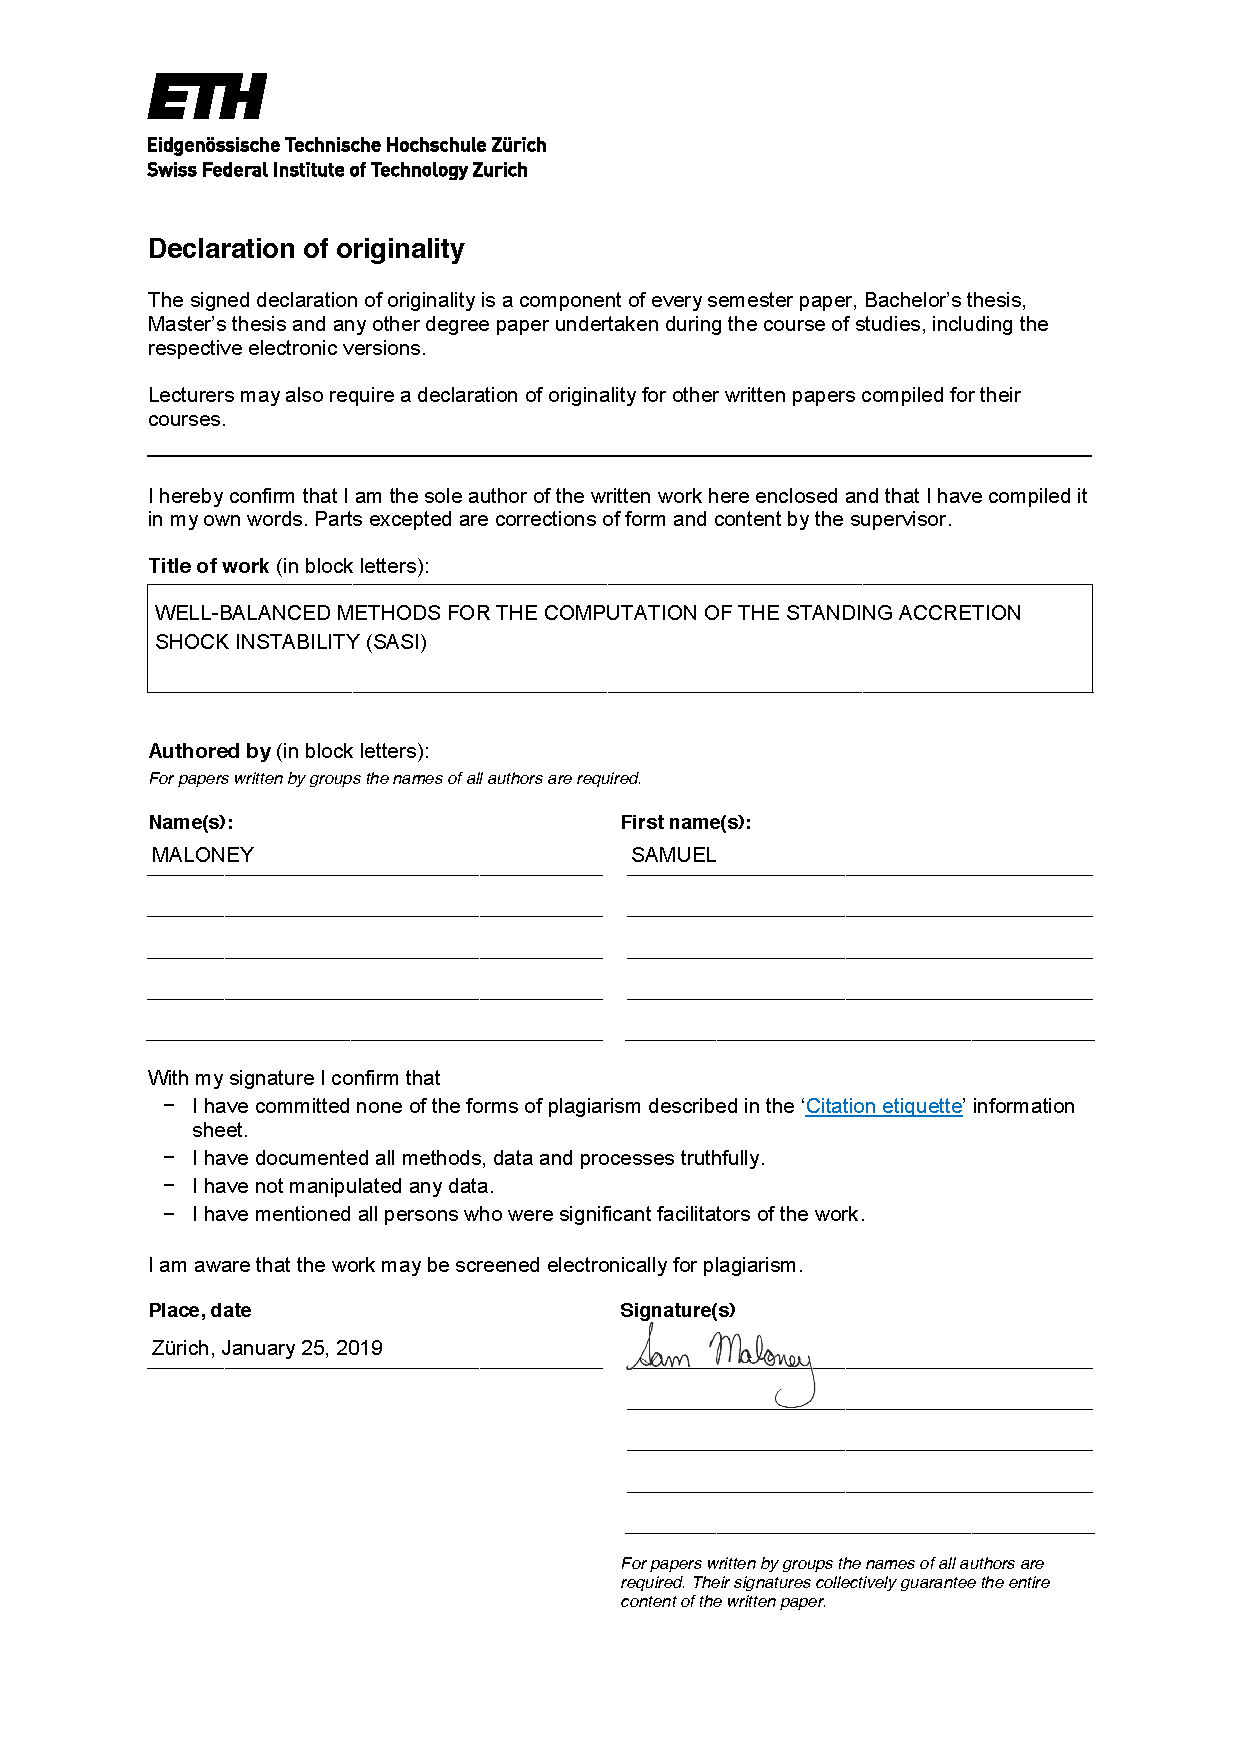
\includepdf[pages={-}]{declaration-originality.pdf}

\end{document}
